\section{Exercises}

%%%%%%%%%%%%%%%%%%%%%%

\subsection{Paired data}

%%%%%%%%%%%%%%%%%%%%%%

% 1

%{\dph{
\eoce{Is there strong evidence that the continental U.S. is warming? We might take a simple approach to this problem and compare how temperatures have changed from 1968 to 2008. The daily high temperature reading on January 1 was collected for 1968 and 2008 for 51 randomly selected locations in the continental U.S. Then the difference between the two readings (temperature in 2008 - temperature in 1968) was calculated for each of the 51 different locations. The average of these 51 values was 1.1 degrees with a standard deviation of 4.9 degrees. We are interested in finding whether these data provide strong evidence of temperature warming in the continental U.S. 
\begin{enumerate}[(a)]
\setlength{\itemsep}{0mm}
\item Are the two data sets of 51 observations dependent or independent of each other? Based on this, what type of analysis should be conducted to test if these data provide strong evidence of temperature warming in the continental U.S?
\item Write the hypotheses in symbols and in words.
\item Calculate the test statistic and find the p-value. (Reminder: check assumptions and conditions.)
\item What do you conclude? Interpret your conclusion in context.
\item What type of error might we have made? Explain in context what the error means.
\item Based on the result of this hypothesis test, would you expect a confidence interval for the average difference between the temperature measurements from 1968 and 2008 to include 0? Explain your reasoning.
\end{enumerate}
}
{
\begin{enumerate}[(a)]
\item The observations in the two data sets are dependent since they are recorded at the same location; therefore, a hypothesis test for paired data should be used for this analysis.
\item $H_0: \mu_{diff} = 0$ (There is no difference in average daily high temperature between January 1, 1968 and January 1, 2008) \\
$H_0: \mu_{diff} > 0$ (Average daily high temperature in January 1, 1968 was lower than average daily high temperature in January, 2008.)
\item Before calculating the test statistic we should check that the assumptions and conditions are satisfied. 
\begin{enumerate}[1.]
\item Independence Assumption: 
\begin{itemize}
\item Random Sampling Condition: We are told that locations are sampled randomly.
\item 10\% Condition: 51 $<$ 10\% of all possible locations we could collect such measurements in the continental U.S.
\end{itemize}
Since we have a random sample and the 10\% condition is satisfied, we can assume that the temperature in one location is independent of another.
\item Nearly Normal Condition: As long as the distributions of the daily high temperatures on January 1 on 1968 and 2008 are not extremely skewed, $n > 50$ should be large enough to assume that the both sample means are normally distributed.
\item Dependent Groups: The two samples are dependent on each other. \\
\end{enumerate}
The test statistic and the p-value can be calculated as follows:
\[ Z = \frac{\bar{x}_{diff} - \mu_{diff}}{ \frac{s_{diff}}{\sqrt{n}} } = \frac{1.1 - 0}{\frac{4.9}{\sqrt{51}}} = \frac{1.1}{0.6861} = 1.60 \]
\[ p-value = P(Z > 1.60) = 1 - 0.9452 = 0.0548 \]
\item Since the p-value $> \alpha$ (since not given use 0.05), fail to reject $H_0$. The data do not provide strong evidence of temperature warming in the continental U.S. However it should be noted that the p-value is very close to 0.05.
\item Type II, since we may have incorrectly failed to reject $H_0$. If we made such an error and concluded that there isn't strong evidence for temperature warming in the continental U.S., but in reality average temperature on January 1, 2008 is significantly higher than average temperature on January 1, 1968.
\item Since we failed to reject $H_0$ which claimed the average difference is equal to 0, we would expect a confidence interval to include this value.
\end{enumerate}
}\label{temperatureWarming}
%}
%}

% 2

{
\eoce{During Exercise~\eoceref{temperatureWarming}, we considered the differences between the temperature readings in January 1 of 1968 and 2008 at 51 locations in the continental U.S.
\begin{enumerate}[(a)]
\setlength{\itemsep}{0mm}
\item Calculate a 90\% confidence interval for the average difference between the temperature measurements between 1968 and 2008.
\item Interpret this interval in context.
\item Does this interval agree with the conclusion of the hypothesis test from Exercise~\eoceref{temperatureWarming}? Explain.
\end{enumerate}
}
{
\begin{enumerate}[(a)]
\item A 90\% confidence interval can be calculated as follows:
\begin{align*}
\bar{x}_{diff} \pm z^{\star} \frac{s_{diff}}{\sqrt{n}} &= 1.1 \pm 1.65 \frac{4.9}{\sqrt{51}} \\
&= 1.1 \pm 1.65 * 0.6861 \\
&= 1.1 \pm 1.13 \\
&= (-0.03, 2.23)
\end{align*}
\item We are 90\% confident that the average daily high in January 1, 2008 in the continental U.S. was 0.13 degrees lower to 2.13 degrees higher than the average daily high in January 1, 1968.
\item Yes, we failed to reject $H_0$ which claimed the average difference is equal to 0, and the interval includes this value.
\end{enumerate}
}
}

%

\pagebreak
\subsection{Difference of two means}

% 3

\eoce{In 1964 the Office of the Surgeon General released their first report linking smoking to various health issues, including cancer. Research done by an ad agency surveyed the number of cigarettes smoked by 80 smokers the day before the Surgeon General�s report came out. The sample average was 13.5 and the standard deviation was 3.2. A year after the report was released, in a random sample of 85 smokers, the average number of cigarettes smoked per day was 12.6 with a standard deviation of 2.9. Is there strong evidence that the average number of cigarettes smoked per day decreased after the Surgeon General's report?

\begin{center}
\begin{tabular}{c|cc}
 & Before & After \\
\hline
n & 80 & 85 \\
$\bar{x}$ & 13.5 & 12.6 \\
s & 3.2 & 2.9
\end{tabular}
\end{center}

\begin{enumerate}[(a)]
\setlength{\itemsep}{0mm}
\item Write the hypotheses in symbols and in words.
\item Calculate the test statistic and find the p-value. (Reminder: check assumptions and conditions.)
\item What do you conclude? Interpret your conclusion in context.
\item Does this imply that the Surgeon General's report was the cause of this decrease? Explain.
\item What type of error might we have made? Explain.
\end{enumerate}
}
{
\begin{enumerate}[(a)]
\item Let $\mu_1$ denote population mean Before, and $\mu_2$ denote population mean After.

$H_0: \mu_1 = \mu_2$, another way to write this is $\mu_1 - \mu_2 = 0$ (The population mean of number of cigarettes smoked per day did not change after the Surgeon General's report) \\
$H_A: \mu_1 > \mu_2$, another way to write this is $\mu_1 - \mu_2 > 0$ (The population mean of number of cigarettes smoked per day decreased after the Surgeon General's report)

\item Before calculating the test statistic we should check that the assumptions and conditions are satisfied. 
\begin{enumerate}[1.]
\item Independence Assumption: 
\begin{itemize}
\item Random Sampling Condition: We are told that the samples are random.
\item 10\% Condition: 80 and 82 $<$ 10\% of smokers in the 1960s.
\end{itemize}
Since we have a random sample and the 10\% condition is satisfied, we can assume that the number of cigarettes smoked by the subjects are independent of each other.
\item Nearly Normal Condition: As long as the distributions of number of cigarettes smoked per day before and after the report was released are not extremely skewed, $n > 50$ should be large enough to assume that the both sample means are normally distributed.
\item Independent Groups: The two samples are independent of each other. \\
\end{enumerate}
The test statistic and the p-value can be calculated as follows:
\[ Z = \frac{(\bar{x}_1 - \bar{x_2}) - (\mu_1 - \mu_2)}{\sqrt{ \frac{s_1^2}{n_1} + \frac{s_2}{n_2} }} = \frac{(13.5 - 12.6) - 0}{ \sqrt{\frac{3.2^2}{80} + \frac{2.9^2}{85}} } = 1.89 \]
\[ p-value = P(z > 1.89) = 1 - 0.9706 = 0.0294 \]

\item Since the p-value $< \alpha$ (since not given use 0.05), reject $H_0$. There is sufficient evidence to suggest that the number of cigarettes smoked per day decreased after the Surgeon General's report.

\item No, we cannot make a causal connection because this is observational data.

\item Type I, since we may have incorrectly rejected $H_0$.

\end{enumerate}
}\label{SterlingCooper}

% 4

\eoce{Based on the data given in Exercise~\eoceref{SterlingCooper}, construct a 90\% confidence interval for the difference between the average number of cigarettes smoked per day before and after the Surgeon General's report was released. Interpret this interval in context. Also comment on if the confidence interval agrees with the conclusion of the hypothesis test from Exercise~\eoceref{SterlingCooper}. 
}
{
A 90\% confidence interval can be calculated as follows:
\begin{align*}
(\bar{x}_1 - \bar{x}_2) \pm z^{\star} \sqrt{ \frac{s_1^2}{n_1} + \frac{s_2^2}{n_2} } &= (13.5 - 12.6) \pm 1.65 * \sqrt{\frac{3.2^2}{80} + \frac{2.9^2}{85}} \\
&= 0.9 \pm 1.65 * 0.4764 \\
&= 0.9 \pm 0.79 \\
&= (0.11, 1.69)
\end{align*}

We are 90\% confident that the average number of cigarettes smoked per day before the report was released is 0.11 to 1.69 higher than the average number of cigarettes smoked after the report was released.

Yes, in Exercise~\eoceref{SterlingCooper} we rejected $H_0$ which claims that the two population means are equal to each other, and the confidence interval does not include 0.
}

% 5

\eoce{The National Assessment of Educational Progress tested 13 year old students in reading in 2004 and 2008. A random sample of 1,000 students who took the test in 2004 yielded an average score of 257 with a standard deviation of 39. A random sample of 1,000 students who took the test in 2008 yielded an average score of 260 with a standard deviation of 38. Construct a 90\% confidence interval for the difference between the average scores in 2004 and 2008. Interpret this interval in context. (Reminder: check assumptions and conditions.)  \citep{web:naep}
}
{
Before constructing the confidence interval we should check that the assumptions and conditions are satisfied. 
\begin{enumerate}[1.]
\item Independence Assumption: 
\begin{itemize}
\item Random Sampling Condition: We are told that both samples are random
\item 10\% Condition: 1,000 $<$ 10\% of all 13 year old students in 2004 an 2008.
\end{itemize}
Since we have a random sample and the 10\% condition is satisfied, we can assume that the how well one student in the sample scores on the exam is independent of another.
\item Nearly Normal Condition: As long as the distribution of scores in 2004 and 2008 are not extremely skewed, such a large sample size should be enough to assume that the both sample means are nearly normally distributed.
\item Independent Groups: Both are random samples from two different years, so we have no reason to think the samples would not be independent of each other.
\end{enumerate}
A 90\% confidence interval can be calculated as follows:
\begin{align*}
(\bar{x}_1 - \bar{x}_2) \pm z^{\star} \sqrt{ \frac{s_1^2}{n_1} + \frac{s_2^2}{n_2} } &= (257 - 260) \pm 1.65 *  \sqrt{\frac{39^2}{1000} + \frac{38^2}{1000}} \\
&= -3 \pm 1.65 * 1.7219 \\
&= -3 \pm 2.84 \\
&= (-5.84, -0.16)
\end{align*}
We are 90\% confident that the average score in 2004 was 0.16 to 5.84 points lower than the average score in 2008.
}\label{mathScore}

% 6

\eoce{Exercise~\eoceref{mathScore} provides data on the average math scores from tests conducted by the National Assessment of Educational Progress in 2004 and 2008.
\begin{enumerate}[(a)]
\item Do these data provide strong information that the average reading score for 13 year old students has changed between 2004 and 2008? Use a 10\% significance level.
\item What type of error might we have made? Explain.
\item Does the conclusion of your hypothesis test agree with the confidence interval from Exercise~\eoceref{mathScore}?
\end{enumerate}
}
{
\begin{enumerate}[(a)]
\item 
$H_0: \mu_{2004} = \mu_{2008} \rightarrow \mu_{2004} - \mu_{2008} = 0$ (Average reading score in 2004 is equal to average reading score in 2008) \\
$H_A: \mu_{2004} \ne \mu_{2008} \rightarrow \mu_{2004} - \mu_{2008} \ne 0$ (Average reading score in 2004 is different than average math score in 2004) \\
Assumptions and conditions have already been checked in Exercise~\eoceref{mathScore}. The test statistic and the p-value can be calculated as follows:
\[ Z = \frac{(\bar{x}_{2004} - \bar{x}_{2008}) - (\mu_{2004} - \mu_{2008})}{\sqrt{ \frac{s_{2004}^2}{n_{2004}} + \frac{s_{2008}}{n_{2008}} }} = \frac{(257 - 260) - 0}{ \sqrt{\frac{39^2}{1000} + \frac{38^2}{1000}} } = \frac{-3}{1.7219} = -1.74 \]
\[ p-value = P(|z| > -1.74) = 2 * 0.0409 = 0.0818 \]
Since the p-value $< \alpha$, reject $H_0$. The data provide strong evidence that the average reading score for 13 year old students has changed between 2004 and 2008.
\item Type I, since we may have incorrectly rejected $H_0$.
\item Yes, we rejected $H_0$ and the confidence interval does not include 0.
\end{enumerate}
}

\pagebreak
% 7

\eoce{Women are said to be obese if they have greater than 35\% body fat, while the cutoff for men being termed obese is 25\%. The cutoff for women is higher since women store extra fat in their bodies to be used during childbearing. The third National Health and Nutrition Examination Survey collected body fat percentage (BF) and lean mass data from 13,601 subjects ages 20 to 79.9. A summary table for these data is given below. Note that BF and lean mass are given as \textit{mean $\pm$ standard error}. Test the hypothesis that women on average have a higher body fat percentage than men using these data. You may assume that all assumptions and conditions for inference are satisfied. \citep{Romero:2008} 
\begin{center}
\begin{tabular}{l c c c}
\hline
Gender	& n		& BF (\%)			& Lean mass (kg)	\\
\hline
Men		& 6580	& 23.9 $\pm$ 0.07	& 61.8 $\pm$ 0.12 \\
Women	& 7021	& 35.0 $\pm$ 0.09	& 44.0 $\pm$ 0.08 \\
\hline
\end{tabular}
\end{center}
Test the hypothesis that women have higher average body fat percentages than men using a 1\% significance level.
}
{
Let $\mu_1$ denote population mean for men, and $\mu_2$ denote population mean for women. 

$H_0: \mu_1 = \mu_2$ (There is no difference between the average BF\% of men and women.) \\
$H_A: \mu_1 < \mu_2$ (Average BF\% of women is higher than average BF\% for men.) 

Before we can do the hypothesis test we must first calculate the standard deviations of the two samples. Remember, $SE = \frac{s}{\sqrt{n}}$. \\
\begin{minipage}[c]{0.5\textwidth}
\begin{center}
Men: 
\begin{align*}
0.07 &= \frac{s}{\sqrt{6580}} \\
s &= 0.07 * \sqrt{6580} = 5.68
\end{align*}
\end{center}
\end{minipage}
\begin{minipage}[c]{0.5\textwidth}
\begin{center}
Women: 
\begin{align*}
0.09 &= \frac{s}{\sqrt{7021}} \\
s &= 0.09 * \sqrt{7021} = 7.54 \\
\end{align*}
\end{center}
\end{minipage}

The test statistic and the p-value can be calculated as follows:
\[ Z = \frac{(\bar{x}_1 - \bar{x_2}) - (\mu_1 - \mu_2)}{\sqrt{ \frac{s_1^2}{n_1} + \frac{s_2}{n_2} }} = \frac{(23.9 - 35.0) - 0}{ \sqrt{\frac{5.68 ^2}{6580} + \frac{7.54 ^2}{7021}} } = -97.35 \]
\[ p-value = P(|z| > -97.35) \approx 0 \]

Since the p-value $< \alpha$, reject $H_0$. The data provide strong evidence that average body fat percentage for women is higher.
}\label{bodyFatMenWomen}

% 8

{\eoce{Exercise~\eoceref{bodyFatMenWomen} also provides information on the amount of lean mass of men and women who were surveyed. Calculate a 95\% confidence interval for the difference between the lean mass amounts of men and women, and interpret the interval in context. Also comment on whether or not this interval suggests a significant difference between the average lean mass amounts of men and women.}
{
Before we can calculate a confidence interval we must first calculate the standard deviations of the two samples. Remember, $SE = \frac{s}{\sqrt{n}}$. \\
\begin{minipage}[c]{0.5\textwidth}
\begin{center}
Men: 
\begin{align*}
0.12 &= \frac{s}{\sqrt{6580}} \\
s &= 0.12 * \sqrt{6580} = 9.73
\end{align*}
\end{center}
\end{minipage}
\begin{minipage}[c]{0.5\textwidth}
\begin{center}
Women: 
\begin{align*}
0.08 &= \frac{s}{\sqrt{7021}} \\
s &= 0.08 * \sqrt{7021} = 6.70 \\
\end{align*}
\end{center}
\end{minipage}
%
A 95\% confidence interval can be calculated as follows:
\begin{align*}
(\bar{x}_1 - \bar{x}_2) \pm z^{\star} \sqrt{ \frac{s_1^2}{n_1} + \frac{s_2^2}{n_2} } &= (61.8 - 44) \pm 1.96 *  \sqrt{\frac{9.73^2}{6580} + \frac{6.70 ^2}{7021}} \\
&= 17.8 \pm 1.96 * 0.1442 \\
&= 17.8 \pm 0.28 \\
&= (17.52, 18.08)
\end{align*}
We are 95\% confident that the average lean mass in men is 17.52 $kg$ to 18.08 $kg$ higher than the average lean mass in women. Since the confidence interval does not include 0, we can infer, at a 5\% significance level, that there is a significant difference between the average lean mass of men and women.
}
}

%%%%%%%%%%%%%%%%%%%%%%

\subsection{Single population proportion}

%%%%%%%%%%%%%%%%%%%%%%

% 9

\eoce{Suppose that 8\% of college students are vegetarians. Determine if the following statements are true or false, and explain your reasoning.
\begin{enumerate}[(a)]
\setlength{\itemsep}{0mm}
\item The distribution of the sample proportions of vegetarians in random samples of size 60 is nearly normal since $n \ge 50$. 
\item The distribution of the sample proportions of vegetarian college students in random samples of size 50 is right skewed.
\item A random sample of 125 college students where 12\% are vegetarians would be considered unusual. 
\item A random sample of 250 college students where 12\% are vegetarians would be considered unusual.
\item The standard error would be reduced by one-half if we increased the sample size from 125 to 250.
\end{enumerate}
}
{
\begin{enumerate}[(a)]
\item FALSE. For the distribution of $\hat{p}$ to be nearly normal, we need to have at least 10 successes and 10 failures in our sample. Unlike with means, for the sampling distribution of proportions to be nearly normal, we need to have at least 10 successes and 10 failures in our sample. We do not use $n \ge 50$ as a condition to check for the normality of the distribution of $\hat{p}$.
\item TRUE. The success-failure condition is not satisfied
\[ np = 50 * 0.08 = 4~and~ n(1 - p) = 50 * 0.92 = 46, \]
therefore we know that the distribution of $\hat{p}$ is not nearly normal. In most samples we would expect $\hat{p}$ to be close to 0.08, the true population proportion. While $\hat{p}$ can be as high as 1 (though we would expect this to happen very rarely), it can only go as low as 0. Therefore the distribution would probably take on a right-skewed shape. Plotting the sampling distribution would confirm this suspicion.
\item FALSE. Standard error of $\hat{p}$ in samples with $n = 125$ can be calculated as:
\[SE_{\hat{p}} = \sqrt{ \frac{p(1-p)}{n} } = \sqrt{\frac{0.08 * 0.92}{125}} = 0.0243 \]
A $\hat{p}$ of 0.12 is only $\frac{0.12 - 0.08}{0.0243} = 1.65$ standard errors away from the mean, which would not be considered unusual.
\item TRUE. Standard error of $\hat{p}$ in samples with $n = 125$ can be calculated as:
\[SE_{\hat{p}} = \sqrt{ \frac{p(1-p)}{n} } = \sqrt{\frac{0.08 * 0.92}{250}} = 0.0172 \]
A $\hat{p}$ of 0.12 is only $\frac{0.12 - 0.08}{0.0172} = 2.32$ standard errors away from the mean, which might be considered unusual.
\item FALSE. Since $n$ appears under the square root sign in the formula for the standard error, increasing the sample size from 125 to 250 would decrease the standard error of the sample proportion only by a factor of $\sqrt{2}$.
\end{enumerate}
}

% 10

{
\eoce{Suppose that the proportion of the adult population who jog is 0.15. Determine if the following statements are true or false, and explain your reasoning. 
\begin{enumerate}[(a)]
\setlength{\itemsep}{0mm}
\item The distribution of the proportions of joggers in random samples of size 40 is right skewed.
\item The distribution of the proportions of joggers in random samples of size 80 is nearly normal since $n \ge 50$. 
\item A random sample of 150 where 20\% are joggers would be considered unusual. 
\item A random sample of 300 where 20\% are joggers would be considered unusual.
\item The standard error would be reduced by one-half if we increased the sample size from 150 to 600.
\end{enumerate}
}
{
\begin{enumerate}[(a)]
\item TRUE. The success-failure condition is not satisfied
\[ np = 40 * 0.15 = 6~and~ n(1-p) = 40 * 0.85 = 34, \]
therefore we know that the distribution of $\hat{p}$ is not nearly normal. In most samples we would expect $\hat{p}$ to be close to 0.15, the true population proportion. While $\hat{p}$ can be as high as 1 (thought we would expect this to happen very rarely), it can only go as low as 0. Therefore the distribution would take on a right skewed shape.
\item FALSE. Unlike with means, for the sampling distribution of proportions to be nearly normal, we need to have at least 10 successes and 10 failures in our sample. We do not use $n \ge 50$ as a condition to check for the normality of the distribution of $\hat{p}$.
\item FALSE. Standard error of $\hat{p}$ in samples with $n = 150$ can be calculated as:
\[SE_{\hat{p}} = \sqrt{ \frac{p(1-p)}{n} } = \sqrt{\frac{0.15 * 0.85}{150}} = 0.0292 \]
A $\hat{p}$ of 0.12 is only $\frac{0.22 - 0.15}{0.0357} = 1.71$ standard errors away from the mean, which would not be considered unusual.
\item TRUE. Standard error of $\hat{p}$ in samples with $n = 300$ can be calculated as:
\[SE_{\hat{p}} = \sqrt{ \frac{p(1-p)}{n} } = \sqrt{\frac{0.15 * 0.85}{300}} = 0.0206 \]
A $\hat{p}$ of 0.12 is only $\frac{0.22 - 0.15}{0.0206} = 2.43$ standard errors away from the mean, which might be considered unusual.
\item TRUE. Since $n$ appears under the square root sign in the formula for the standard error, quadrupling the sample size will reduce the standard error by a half.
\end{enumerate}
}
}

% 11

{
\eoce{Ninety percent of orange tabby cats are male. Determine if the following statements are true or false, and explain your reasoning.
\begin{enumerate}[(a)]
\setlength{\itemsep}{0mm}
\item The distribution of sample proportions of samples of size 30 is left skewed.
\item Doubling the sample size will reduce the standard error of the sample proportion by one-half.
\item The distribution of sample proportions of samples of size 140 is approximately normal.
\item Doubling the sample size will reduce the standard error of the sample proportion by a factor of $\sqrt{2}$.
\item The distribution of sample proportions of samples of size 70 is approximately normal.
\end{enumerate}
}
{
\begin{enumerate}[(a)]
\item TRUE. The success-failure condition is not satisfied
\[ n\hat{p} = 30 * 0.90 = 27~and~ n\hat{q} = 30 * 0.10 = 3, \]
therefore we know that the distribution of $\hat{p}$ is not nearly normal. In most samples we would expect $\hat{p}$ to be close to 0.90, the true population proportion. While $\hat{p}$ can be as low as 0 (thought we would expect this to happen very rarely), it can only go as high as 1. Therefore the distribution would probably take on a left-skewed shape. Plotting the sampling distribution would confirm this suspicion.
\item FALSE.  Since $n$ appears under the square root sign in the formula for the standard error, doubling the sample size would decrease the standard error of the sample proportion only by a factor of $\sqrt{2}$.
\item TRUE. The success-failure condition is satisfied
\[ n\hat{p} = 140 * 0.90 = 126 ~and~ n\hat{q} = 140 * 0.10 = 14, \]
therefore the distribution of $\hat{p}$ is nearly normal.
\item TRUE. 
\[ SE_{old} =  \sqrt{\frac{\hat{p}\hat{q}}{n}} ~\hspace{1cm}~ SE_{new} = \sqrt{\frac{\hat{p}\hat{q}}{2n}} = \frac{1}{\sqrt{2}} \sqrt{\frac{\hat{p}\hat{q}}{n}} = \frac{1}{\sqrt{2}}ME_{old}\]
\item FALSE. The success-failure condition is not satisfied
\[ n\hat{p} = 70 * 0.90 = 63 ~and~ n\hat{q} = 70 * 0.10 = 7, \]
therefore the distribution of $\hat{p}$ is not nearly normal.
\end{enumerate}
}
}

% 12

{
\eoce{In a poll conducted by Survey USA on July 12, 2010, 70\% of the 119 respondents between the ages of 18 and 34 said they would vote in the 2010 general election for Prop 19, which would change California law to legalize marijuana and allow it to be regulated and taxed. At a 95\% confidence level, this sample has an 8\% margin of error. Based on this information, determine if the following statements are true or false, and explain your reasoning.
\begin{enumerate}[(a)]
\setlength{\itemsep}{0mm}
\item We are 95\% confident that between 62\% and 78\% of the California voters in this sample support Prop 19.
\item We are 95\% confident that between 62\% and 78\% of all California voters between the ages of 18 and 34 support Prop 19.
\item If we considered many random samples of 119 California voters between the ages of 18 and 34, and we calculated the sample proportions of those who support Prop 19, 95\% of them will be between 62\% and 78\%.
\item In order to decrease the margin of error to 4\%, we would need to quadruple (multiply by 4) the sample size.
\item Based on this confidence interval, there is sufficient evidence to conclude that a majority of California voters between the ages of 18 and 34 support Prop 19.
\end{enumerate}
}
{
\begin{enumerate}[(a)]
\item FALSE. A confidence interval is constructed to estimate the population proportion, not the sample proportion.
\item TRUE. This is the correct interpretation of the confidence interval, which can be calculated as $0.70 \pm 0.08 = (0.62, 0.78)$.
\item FALSE. The confidence interval does not tell us what we might expect to see in another random sample.
\item TRUE. Since the sample size appears under the square root sign in calculation of the standard error, in order to halve the margin of error we would need to quadruple the sample size.
\[ ME_{old} =  z^{\star} \sqrt{\frac{\hat{p}(1 - \hat{q})}{n}} ~\hspace{1cm}~ ME_{new} = z^{\star} \sqrt{\frac{\hat{p}(1 - \hat{p})}{4n}} = z^{\star} \frac{1}{2} \sqrt{\frac{\hat{p}\hat{q}}{n}} = \frac{1}{2}ME_{old}\]
\item TRUE. The confidence interval lies above 50\%.
\end{enumerate}
}
}

% 13

\eoce{We are interested in estimating the proportion of graduates at a mid-sized university who found a job within one year of completing their undergraduate degree. We conduct a survey and find out that 348 of the 400 randomly sampled graduates found jobs. The graduating class under consideration included approximately 4500 students.
\begin{enumerate}[(a)]
\setlength{\itemsep}{0mm}
\item Describe the population parameter of interest. What is the value of the point estimate of this parameter?
\item Construct a 95\% confidence interval for the proportion of graduates who found a job within one year of completing their undergraduate degree at this university. (Reminder: check assumptions and conditions.)
\item Explain what this interval means in the context of this question.
\item What does ``95\% confidence" mean?
\item Without doing any calculations, describe what would happen to the confidence interval if we decided to use a higher confidence level.
\item Without doing any calculations, describe what would happen to the confidence interval if we used a larger sample.
\end{enumerate}
}
{
\begin{enumerate}[(a)]

\item The population parameter of interest is the proportion of all graduates from this university who found a job within one year of graduating, $p$. The point estimate of this parameter is the proportion of graduates in the sample who found a job within one year of graduating, $\hat{p} = \frac{348}{400} = 0.87$. 

\item  Before constructing the confidence interval we should check that the assumptions and conditions are satisfied. 
\begin{enumerate}[1.]
\item Independence Assumption: 
\begin{itemize}
\item Random Sampling Condition: We are told that the sample is random.
\item 10\% Condition: We can safely assume that $400$ $<$ 10\% of all students at a mid-sized university.
\end{itemize}
Since we have a random sample and the 10\% condition is satisfied, we can assume that whether or not one student in the sample has found a job is independent of another.
\item Nearly Normal Condition: First we must check if the success failure condition is met.
\begin{align*}
n\hat{p} &\ge 10 \rightarrow 400 * 0.87 = 348 > 10 \checkmark \\
n(1 - \hat{p}) &\ge 10 \rightarrow 400 * 0.13 = 52 > 10 \checkmark
\end{align*}
Since the observations are independent and the success-failure condition is met, we can assume that $\hat{p}$ is nearly normal. \\
\end{enumerate}
A 95\% confidence interval can be calculated as follows:
\begin{align*}
\hat{p} \pm z^{\star} \sqrt{ \frac{\hat{p} (1 - \hat{p})}{n} } &= 0.87 \pm 1.96 \times \sqrt{\frac{0.87 \times 0.13}{400}} \\
&= 0.87 \pm 0.033 \\
&= (0.837 , 0.903)
\end{align*}

\item We are 95\% confident that the true proportion of graduates from this university who found a job within one year of completing their undergraduate degree is between 83.7\% and 90.3\%.

\item 95\% of random samples of 400 would produce a confidence interval that includes the true proportion of students at this university who found a job within one year of graduating from college.

\item  Increasing the confidence level would increase the margin of error hence widen the interval.

\item Increasing the sample size would decrease the margin of error hence make the interval narrower.

\end{enumerate}
}

% 14

\eoce{After implementing a study abroad program, a university conducted a study to find out what percent of students had already traveled to another country. The survey showed that 42 out of 100 sampled students had previously visited abroad.
\begin{enumerate}[(a)]
\setlength{\itemsep}{0mm}
\item Describe the population parameter of interest. What is the value of the point estimate of this parameter?
\item Construct a 90\% confidence interval for the proportion of students at this university who have traveled abroad. (Reminder: check assumptions and conditions.)
\item Interpret this interval in context.
\item What does ``90\% confidence" mean?
\end{enumerate}
}
{
\begin{enumerate}[(a)]

\item The population parameter of interest is the proportion of all students at this university who have traveled abroad, $p$. The point estimate is the proportion of people in the sample who have traveled abroad, $\hat{p} = 0.42$. 

\item Before constructing the confidence interval we should check that the assumptions and conditions are satisfied. 
\begin{enumerate}[1.]
\item Independence Assumption: 
\begin{itemize}
\item Random Sampling Condition: We are told that the sample is random.
\item 10\% Condition: We can safely assume that $100$ $<$ 10\% of all students at a university.
\end{itemize}
Since we have a random sample and the 10\% condition is satisfied, we can assume that whether or not one student in the sample has traveled abroad is independent of another.
\item Nearly Normal Condition: First we must check if the success failure condition is met.
\begin{align*}
n\hat{p} &\ge 10 \rightarrow 100 * 0.42 = 42 > 10 \checkmark \\
n(1 - \hat{p}) &\ge 10 \rightarrow 100 * 0.58 = 58 > 10 \checkmark
\end{align*}
Since the observations are independent and the success-failure condition is met, we can assume that $\hat{p}$ is nearly normal. \\
\end{enumerate}
A 90\% confidence interval for the proportion of students at this university who have traveled abroad can be calculated as follows:
\begin{align*}
\hat{p} &\pm z^{\star} \sqrt{ \frac{\hat{p} (1 - \hat{p})} {n} } \\
0.42 &\pm 1.65 \sqrt{ \frac{0.42 * 0.58}{100}} \\
0.42 &\pm 1.65 *  0.0494 \\
0.42 &\pm 0.08 \\
(0.34&, 0.50)
\end{align*}

\item We are 90\% confident that 34\% to 50\% of the students at this university have traveled abroad.

\item 90\% of random samples of 100 would produce a confidence interval that includes the true proportion of students at this university who have traveled abroad.

\end{enumerate}
}\label{univTravelAbroad}

% 15

\eoce{It is believed that large doses of acetaminophen (the active ingredient in over the counter pain relievers like Tylenol) may cause damage to the liver. A researcher wants to conduct a study to estimate the proportion of acetaminophen users who have liver damage. For participating in this study, she will pay each subject \$20 and provide a free medical consultation if the patient has liver damage.
\begin{enumerate}[(a)]
\setlength{\itemsep}{0mm}
\item If she wants to limit the margin of error of her 98\% confidence interval to 2\%, what is the minimum amount of money she needs to set aside to pay her subjects?
\item The amount you calculated in part (a) is substantially over her budget so she decides to use fewer subjects. How will this affect the width of her confidence interval.
\end{enumerate}
}
{
\begin{enumerate}[(a)]
\item We are asked to solve for the sample size required to achieve a 2\% margin of error. Since we are not given information from a previous study to use as an estimate for $\hat{p}$, we use 0.5 as it will yield the most conservative estimate.
\begin{align*}
ME = z^{\star} \sqrt{ \frac{\hat{p} (1-\hat{p})} {n} } \rightarrow 0.02 &\ge 2.326 \sqrt{ \frac{0.5 * 0.5} {n} } \\
0.02^2 &\ge 2.33^2  \frac{0.5 * 0.5}{n} \\
n &\ge \frac{2.33^2 * 0.5 * 0.5}{0.02^2} \\
n &\ge 3393.062 \\
n &\ge 3,394
\end{align*}

She needs a minimum of 3,394 subjects and therefore needs to set aside a minimum of $\$3,394 \times 20 = \$67,880$. 

\item Decreasing the sample size would increase the margin of error hence make the interval wider, i.e. the interval would lose precision.

\end{enumerate}
}

% 16

\eoce{We are interested in estimating the proportion of students at a university who smoke. Out of a random sample of 200 students from this university, 40 students smoke. 
\begin{enumerate}[(a)]
\setlength{\itemsep}{0mm}
\item Construct a 95\% confidence interval for the proportion of students at this university who smoke, and interpret this interval in context.
\item Construct a 99\% confidence interval for the proportion of students at this university who do not smoke, and interpret this interval in context. 
\item Compare the widths of the 95\% and 99\% confidence intervals. Which one is wider? Can you explain why this is the case?
\item If we wanted the margin of error to be no larger than 2\% for at a 95\% confidence level for the proportion of students who smoke, how big of a sample would we need? 
\end{enumerate}
}
{
\begin{enumerate}[(a)]
\item Before constructing the confidence interval we should check that the assumptions and conditions are satisfied. 
\begin{enumerate}[1.]
\item Independence Assumption: 
\begin{itemize}
\item Random Sampling Condition: We are told that the sample is random.
\item 10\% Condition: We can safely assume that 200 $<$ 10\% of all students at a university.
\end{itemize}
Since we have a random sample and the 10\% condition is satisfied, we can assume that whether or not not one student smokes is independent of the smoking status of another student in this sample.
\item Nearly Normal Condition: First we must check if the success failure condition is met.
\begin{align*}
n\hat{p} &\ge 10 \rightarrow 200 * 0.2 = 40 > 10 \checkmark \\
n(1 - \hat{p}) &\ge 10 \rightarrow 200 * 0.8 = 160 > 10 \checkmark
\end{align*}
Since the observations are independent and the success-failure condition is met, we can assume that $\hat{p}$ is nearly normal. \\
\end{enumerate}
A 95\% confidence interval can be calculated as follows:
\begin{align*}
\hat{p} &= \frac{40}{200} = 0.2 \\
\hat{p} \pm z^{\star} \sqrt{\frac{\hat{p} (1 - \hat{p})}{n}} &= 0.2 \pm 1.96 * \sqrt{\frac{0.2*0.8}{200}} \\
&= 0.2 \pm 0.055 \\
&= (0.145 , 0.255)
\end{align*}
We are 95\% confident that 14.5\% to 25.5\% of all students at this university smoke.

\item A 99\% confidence interval can be calculated as follows:
\begin{align*}
\hat{p}  &= \frac{200-40}{200} = 0.8 \\
\hat{p} \pm z^{\star} \sqrt{\frac{\hat{p} (1 - \hat{p})}{n}} &= 0.8 \pm  2.576 * \sqrt{\frac{0.8*0.2}{200}} \\
&= .8 \pm .07 \\
&= (0.73 , 0.87)
\end{align*}
We are 99\% confident that 73\% to 87\% of all students at this university do not smoke.

\item The width of the 95\% confidence interval is $0.255 - 0.145 = 0.11$ and the width of the 99\% confidence interval is $0.87 - 0.73 = 0.14$. Since these intervals are based on the same data, i.e. sample sizes are the same, increasing the confidence level decreases the precision.

\item We are asked to solve for the sample size required to achieve a 2\% margin of error. 
\begin{align*}
ME = z^{\star} \sqrt{ \frac{\hat{p} (1-\hat{p})} {n} } \rightarrow 0.02 &= 1.96 \sqrt{ \frac{0.2 * 0.8} {n} } \\
0.02^2 &= 1.96^2  \frac{0.2 * 0.8}{n} \\
n &= \frac{1.96^2 * 0.2 * 0.8}{0.02^2} \\
n &= 1536.64 \approx 1537
\end{align*}

\end{enumerate}
}\label{UnivSmoke}

% 17

{
\eoce{In January 2011, The Marist Poll published a report stating that 66\% of adults nationally think licensed drivers should be required to re-take their road test once they reach 65 years of age. It was also reported that interviews were conducted on 1,018 American adults, and that the margin of error was 3\% using a 95\% confidence level. \citep{maristRoadTest}
\begin{enumerate}[(a)]
\setlength{\itemsep}{0mm}
\item Verify the margin of error reported by The Marist Poll. The data collected was based on simple random sampling.
\item Does the poll contain strong evidence that more than two thirds of the population think that licensed drivers should be required to re-take their road test once they turn 65?
\end{enumerate}
}
{
\begin{enumerate}[(a)]
\item The margin of error can be calculated as follows:
\[ ME = z^{\star} \sqrt{ \frac{\hat{p} (1-\hat{p})} {n} } = 1.96 \sqrt{ \frac{0.66 * 0.34}{1018} }= 0.029 \approx 3\% \]
\item A 95\% confidence interval for the proportion of adults who think that licensed drivers should be required to re-take their road test once they reach 65 years of age can be calculated as
\[ 0.66 \pm 0.03 = (0.63,0.69). \]
Since two thirds (roughly 67\%) is contained in the interval we wouldn't reject a null hypothesis of $H_0$: $p = 0.47$. Therefore, the data do not provide evidence that more than two thirds of the population think that drivers over the age of 65 should re-take their road test.
\end{enumerate}
}}

\pagebreak
% 18

\eoce{Exercise~\eoceref{univTravelAbroad} provides the result of a campus wide survey where 42 of 100 randomly sampled students have traveled abroad. A comprehensive follow-up survey was conducted one year after the study abroad program was implemented. It sampled all students at the university and found that 51\% of the university's students had traveled to another country. Do you think there has been an increase in the number of students who traveled abroad since the first survey? Conduct a hypothesis test to check. Would you come to the same conclusion using your confidence interval from Exercise~\eoceref{univTravelAbroad}?
}
{
$H_0: p = 0.51$(51\% of students at this university have traveled
 abroad) \\
$H_A: p < 0.51$ (Less than 51\% of students at this university have traveled
 abroad)

We have shown in Exercise~\eoceref{univTravelAbroad} that assumptions and conditions for inference are satisfied. However we need to re-check the success failure condition since in hypothesis testing we use $p$ instead of $\hat{p}$ when checking this condition.
\[ 100 * 0.51 = 51 > 10 \checkmark \qquad 100 * 0.49 = 49 > 10 \checkmark \]

\begin{minipage}[c]{0.45\textwidth}
\begin{align*}
Z &= \frac{\hat{p} - p_0}{\sqrt{\frac{p_0 (1 - p_0)}{n}}} \\
&= \frac{0.42 - 0.51}{\sqrt{ \frac{0.42 (1 - 0.42)} {100} }} \\
&= \frac{-0.09}{0.0494} = -1.82 \\
p-value &= P(\hat{p} < 0.42 | p = 0.51) \\
&= P(z < -1.82) = 0.0344
\end{align*}
Since the p-value $> \alpha$ (since not given use 0.05), fail to reject $H_0$. \\
\end{minipage}
\begin{minipage}[c]{0.05\textwidth}
$\:$
\end{minipage}
\begin{minipage}[c]{0.5\textwidth}
\begin{center}
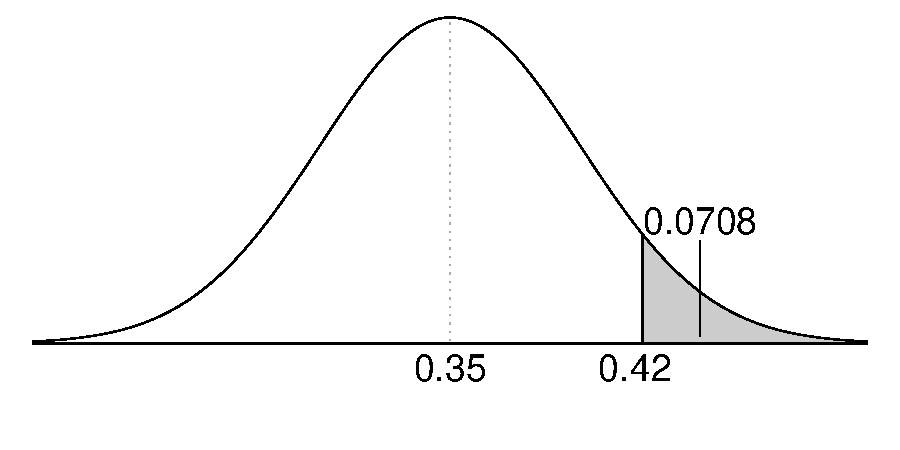
\includegraphics[width=70mm]{05/figures/eoce/abroad}
\end{center}
The data do provide strong evidence that the proportion of students at this university who have traveled
 abroad has increased after the implementation of the study abroad program.
\end{minipage}
We would arrive at the same conclusion using the confidence interval from Exercise~\eoceref{univTravelAbroad} since we rejected the null hypothesis which claims $p = 0.51$ and this value is not included in the confidence interval.
}

% 19

{
\eoce{A national survey conducted in 2011 among a simple random sample of 1,507 adults shows that 56\% of Americans think the Civil War is still relevant to American politics and political life. \citep{civilWar} 
\begin{enumerate}[(a)]
\setlength{\itemsep}{0mm}
\item Conduct a hypothesis test to determine if these data provide strong evidence that majority of the Americans think the Civil War is still relevant.
\item Interpret the p-value in context.
\item Calculate a 90\% confidence interval for the proportion of Americans who think the Civil War is still relevant. Interpret the interval in context and comment on whether or not the confidence interval agrees with the conclusion of the hypothesis test.
\end{enumerate}
}
{
\begin{enumerate}[(a)]
\item $H_0: p = 0.5$ (50\% of Americans think the Civil War is still relevant) \\
$H_A: p > 0.5$ (More than 50\% of Americans think the Civil War is still relevant) \\
Before calculating the test statistic we should check that the assumptions and conditions are satisfied. 
\begin{enumerate}[1.]
\item Independence Assumption: 
\begin{itemize}
\item Random Sampling Condition: We can assume that the sample is random.
\item 10\% Condition: $1,507 $ $<$ 10\% of all Americans.
\end{itemize}
Since we have a random sample and the 10\% condition is satisfied, we can assume that whether or not one American in the sample thinks the Civil War is still relevant is independent of another.
\item Nearly Normal Condition: 
\[ 1,507 * 0.56 = 843.92 > 10 \checkmark \qquad 1,507 * 0.44 = 663.08 > 10 \checkmark \]
Since the observations are independent and the success-failure condition is met, we can assume that $\hat{p}$ is nearly normal.
\end{enumerate}
The test statistic and the p-value can be calculated as follows:
\begin{align*}
Z &= \frac{\hat{p} - p_0}{\sqrt{\frac{p_0 (1 - p_0)}{n}}} = \frac{0.56 - 0.5}{\sqrt{\frac{0.5 * 0.5}{1,507}}} = 4.66 \\
p-value &= P(\hat{p} >  0.56 | p = 0.5) = P(z > 4.66) \approx 0
\end{align*}
Since the p-value is very small, we reject $H_0$. The data provide strong evidence that majority of the Americans think the Civil War is still relevant.
\item If in fact only 50\% of Americans thought the Civil War is still relevant, the probability of obtaining a ransom sample of 1,507 Americans where 56\% or more think it is still relevant would be approximately 0.
\item A 90\% confidence interval can be calculated as follows:
\begin{align*}
\hat{p} \pm z^{\star} \sqrt{\frac{\hat{p} (1 - \hat{p})}{n}} &= 0.56 \pm 1.65 * \sqrt{\frac{0.56 * 0.44}{1,507}} \\
&= 0.56 \pm 1.65 * 0.0128 \\
&= 0.56 \pm 0.02 \\
&= (0.54, 0.58)
\end{align*}
We are 90\% confident that 54\% to 58\% of all Americans think that the Civil War is still relevant. This agrees with the conclusion of the earlier hypothesis test since the interval lies above 50\%.
\end{enumerate}
}
}

% 20

\eoce{A college review magazine states that in many business schools there is a certain stigma that marketing is a less stressful major and so most students ($>$50\%) majoring in marketing also major in finance, economics or accounting to be able to show employers that their quantitative skills are also strong. In order to test this claim, an education researcher collects a simple random sample of 80 undergraduate students majoring in marketing at various business schools and finds that 50 of them have a double major.
\begin{enumerate}[(a)]
\setlength{\itemsep}{0mm}
\item Conduct a hypothesis test to determine if these data provide strong evidence supporting this magazine's claim that majority of marketing students have a double major.
\item Interpret the p-value in context.
\item Calculate a 90\% confidence interval for the proportion of marketing students who have a double major. Interpret the interval in context and comment on whether or not the confidence interval agrees with the conclusion of the hypothesis test.
\end{enumerate}
}
{
\begin{enumerate}[(a)]
\item $H_0: p = 0.5$ (50\% of all marketing majors have a double major) \\
$H_A: p > 0.5$ (More than 50\% of all marketing majors have a double major) 

Before calculating the test statistic we should check that the assumptions and conditions are satisfied. 
\begin{enumerate}[1.]
\item Independence Assumption: 
\begin{itemize}
\item Random Sampling Condition: We are told that the sample is random.
\item 10\% Condition: We can safely assume that $80$ $<$ 10\% of all undergraduate marketing majors.
\end{itemize}
Since we have a random sample and the 10\% condition is satisfied, we can assume that whether or not one student in the sample has a double major is independent of another.
\item Nearly Normal Condition: 
\[ 80 * 0.5 = 40 > 10 \checkmark \qquad 80 * 0.5 = 40 > 10 \checkmark \]
Since the observations are independent and the success-failure condition is met, we can assume that $\hat{p}$ is nearly normal.
\end{enumerate}
The test statistic can be calculated as follows:
\begin{align*}
\hat{p} &= \frac{50}{80} = 0.625 \\
Z &= \frac{\hat{p} - p_0}{\sqrt{\frac{p_0 (1 - p_0)}{n}}} = \frac{0.625 - 0.5}{\sqrt{\frac{0.5 * 0.5}{80}}} = 2.24 \\
p-value &= P(\hat{p} > 0.625 | p = 0.5) = P(z > 2.24) = 1 - 0.9875 = 0.025
\end{align*}
Since the p-value $< \alpha$ (since not given use 0.05), we reject $H_0$. The data provide strong evidence that majority of marketing students have a double major.
\item If in fact half of all marketing students have a double major, the probability of getting a random sample of 80 marketing students where more than 50 have a double major would be 0.025.
\item A 90\% confidence interval can be calculated as follows:
\begin{align*}
\hat{p} \pm z^{\star} \sqrt{\frac{\hat{p} (1 - \hat{p})}{n}} &= 0.625 \pm 1.65 * \sqrt{\frac{0.625 * 0.375}{80}} \\
&= 0.625 \pm 1.65 * 0.048 \\
&= 0.625 \pm 0.08 \\
&= (0.545, 0.725)
\end{align*}
We are 90\% confident that the 54.5\% to 72.5\% of all undergraduate marketing students have a double major. This agrees with the conclusion of the earlier hypothesis test since the interval lies above 50\%.
\end{enumerate}
}\label{DoubleMajor}

% 21

{
\eoce{Among a simple random sample of 331 American adults who do not have a four-year college degree and are not currently enrolled in school, 48\% said they decided to not go to college because they could not afford school. \citep{collegeWorthIt}
\begin{enumerate}[(a)]
\item A newspaper article states that only a minority of the Americans who decide not to go to college do so because they cannot afford it, and uses the point estimate from this survey as evidence. Conduct a hypothesis test to determine if these data provide strong evidence supporting this statement. Use a 10\% significance level.
\item Would you expect a confidence interval for the proportion of American adults who decide to not go to college because they cannot afford it to include 0.5? Explain.
\end{enumerate}
}
{
\begin{enumerate}[(a)]
\item $H_0: p = 0.5$ (50\% of Americas who decide to not go to college because they cannot afford it do so because they cannot afford it) \\
$H_A: p < 0.5$ (Less than 50\% of Americas who decide to not go to college because they cannot afford it do so because they cannot afford it) \\
Before calculating the test statistic we should check that the assumptions and conditions are satisfied. 
\begin{enumerate}[1.]
\item Independence Assumption: 
\begin{itemize}
\item Random Sampling Condition: We are told that the sample is representative.
\item 10\% Condition: We can safely assume that $331$ $<$ 10\% of all American adults who decide to not go to college.
\end{itemize}
Since we have a random sample and the 10\% condition is satisfied, we can assume that whether or not one person in the sample decided to not go to college because they can't afford it is independent of another.
\item Nearly Normal Condition: 
\[ 331 * 0.5 = 165.5 > 10 \checkmark \qquad 331 * 0.5 = 165.5 > 10 \checkmark \]
Since the observations are independent and the success-failure condition is met, we can assume that $\hat{p}$ is nearly normal.
\end{enumerate}
The test statistic can be calculated as follows:
\begin{align*}
Z &= \frac{\hat{p} - p_0}{\sqrt{\frac{p_0 (1 - p_0)}{n}}} = \frac{0.48 - 0.5}{\sqrt{\frac{0.5 * 0.5}{331}}} = -0.73 \\
p-value &= P(\hat{p} < 0.48 | p = 0.5) = P(z < -0.73) = 0.2327
\end{align*}
Since the p-value is large, we fail to reject $H_0$. The data do not provide strong evidence that less than half of American adults who decide to not go to college make this decision because they cannot afford college.
\item Yes, since we failed to reject $H_0$.
\end{enumerate}
}\label{collegeWorthIt}
}

\pagebreak
% 22

\eoce{A \textit{Washington Post} article reports that ``support for a government-run health-care plan to compete with private insurers has rebounded from its summertime lows and wins clear majority support from the public." More specifically, the article says ``seven in 10 Democrats back the plan, while almost nine in 10 Republicans oppose it. Independents divide 52 percent against, 42 percent in favor of the legislation." There were were 819 Democrats, 566 Republicans and 783 Independents surveyed. \citep{WashingtonPost}
\begin{enumerate}[(a)]
\setlength{\itemsep}{0mm}
\item A political pundit on TV claims that a majority of Independents oppose the public option health care plan. Do these data provide strong evidence to support this statement?
\item Would you expect a confidence interval for the proportion of Independents who oppose the public option plan to include 0.5? Explain.
\end{enumerate}
}
{
\begin{enumerate}[(a)]

\item $H_0: p = 0.50$ (50\% of all Independents are oppose the public option plan) \\
$H_A:  p > 0.50$ (More than 50\% of all Independents are oppose the public option plan)

Before calculating the test statistic we should check that the assumptions and conditions are satisfied. 
\begin{enumerate}[1.]
\item Independence Assumption: 
\begin{itemize}
\item Random Sampling Condition: We are told that the sample is random.
\item 10\% Condition: 783 $<$ 10\% of all Independents.
\end{itemize}
Since we have a random sample and the 10\% condition is satisfied, we can assume that whether or not one independent opposes the plan is independent of whether or not another one does.
\item Nearly Normal Condition: 
\[ 783 * 0.50 = 391.5 > 10 \checkmark \qquad 783 * 0.50 = 391.5 > 10 \checkmark \]
Since the observations are independent and the success-failure condition is met, we can assume that $\hat{p}$ is nearly normal.
\end{enumerate}
The test statistic can be calculated as follows:
\begin{align*}
\hat{p} &= 0.52 \\
Z &= \frac{\hat{p} - p_0}{\sqrt{\frac{p_0q_0}{n}}} = \frac{0.52 - 0.50}{\sqrt{\frac{0.50 * 0.50}{783}}} = 1.12 \\
p-value &= P(z > 1.12) = 1 - 0.8686 = 0.1314
\end{align*}
Since the p-value $> \alpha$ (use $\alpha = 0.05$ since not given), we fail to reject $H_0$. The data do not provide strong evidence that more than half of all Independents oppose the public option plan.

\item Yes, since we failed to reject $H_0$, which claims that the proportion of Independents who oppose the public option plan equals 0.5, we would expect a confidence interval to include this value.

\end{enumerate}
}\label{WashPost}

% 23

{\eoce{Exercise~\eoceref{collegeWorthIt} presents the results of a poll where 48\% of 331 Americans who decide to not go to college do so because they cannot afford it.
\begin{enumerate}[(a)]
\setlength{\itemsep}{0mm}
\item Construct an 80\% confidence interval for the proportion of Americans who decide to not go to college do so because they cannot afford it. Interpret it in context and comment on whether or not the confidence interval agrees with the conclusion of the hypothesis test from Exercise~\eoceref{collegeWorthIt}.
\item Suppose we wanted the margin of error for the 80\% confidence level to be about 1.5\%. How large of a survey would you recommend?
\end{enumerate}
}
{
\begin{enumerate}[(a)]
\item We have confirmed in Exercise~\eoceref{collegeWorthIt} that the assumptions and conditions are satisfied. An 80\% confidence interval can be calculated as follows:
\begin{align*}
\hat{p} \pm z^{\star} \sqrt{\frac{\hat{p} (1 - \hat{p})}{n}} &= 0.48 \pm 1.28 * \sqrt{\frac{0.48 * 0.52}{331}} \\
&= 0.48 \pm 1.28 * 0.0275 \\
&= 0.48 \pm 0.035 \\
&= (0.445, 0.515)
\end{align*}
We are 80\% confident that the 44.5\% to 51.5\% of all Americans who decide not to go to college do so because they cannot afford it. This agrees with the conclusion of the earlier hypothesis test since the interval includes 50\%.
\item We are asked to solve for the sample size required to achieve a 1.5\% margin of error. 
\begin{align*}
ME = z^{\star} \sqrt{ \frac{\hat{p} (1-\hat{p})} {n} } \rightarrow 0.01 &\ge 1.28 \sqrt{ \frac{0.48 * 0.52} {n} } \\
0.015^2 &\ge 1.28^2  \frac{0.48 * 0.52}{n} \\
n &\ge \frac{1.28^2 * 0.48 * 0.52}{0.015^2} \\
n &\ge 1817.532 \approx 1,818
\end{align*}
\end{enumerate}
}
}

% 24

\eoce{Exercise~\eoceref{WashPost} presents the results of a poll evaluating support for the public option health care plan in 2009.
\begin{enumerate}[(a)]
\setlength{\itemsep}{0mm}
\item Construct an 90\% confidence interval for the proportion of Independents who oppose the public option health care plan. Interpret it in context and comment on whether or not the confidence interval agrees with the conclusion of the hypothesis test from Exercise~\eoceref{WashPost}?
\item If we wanted to limit the margin of error of a 90\% confidence interval to 1\%, about how many Independents would we need to survey?
\end{enumerate}
}
{
\begin{enumerate}[(a)]
\item We have confirmed in Exercise~\eoceref{WashPost} that the assumptions and conditions are satisfied. A 90\% confidence interval can be calculated as follows:
\begin{align*}
\hat{p} \pm z^{\star} \sqrt{\frac{\hat{p} ( 1 - \hat{p})}{n}} &= 0.52 \pm 1.65 *  \sqrt{\frac{0.52 * 0.48}{783}} \\
&= 0.52 \pm 1.65 * 0.0179 \\
&= 0.52 \pm 0.03 \\
&= (0.49, 0.55)
\end{align*}
We are 90\% confident that 49\% to 55\% of Independents oppose the public option plan. This agrees with the conclusion of the earlier hypothesis test since the interval includes 50\%.
\item  We are asked to solve for the sample size required to achieve a 1\% margin of error. 
\begin{align*}
ME = z^{\star} \sqrt{ \frac{\hat{p} (1-\hat{p})} {n} } \rightarrow 0.01 &\ge 1.65 \sqrt{ \frac{0.52 * 0.48} {n} } \\
0.01^2 &\ge 1.65 ^2  \frac{0.52 * 0.48}{n} \\
n &\ge \frac{1.65 ^2 * 0.52 * 0.48}{0.01^2} \\
n &\ge 6,795.36 \\
n &\ge 6,796
\end{align*}
\end{enumerate}
}

% 25

\eoce{A report by the Centers for Disease Control and Prevention states that 30\% of Americans are habitually getting less than six hours of sleep a night -- less than the recommended seven to nine hours. New York is known as ``the city that never sleeps". In a simple random sample of 300 New Yorkers, it was found that 105 of them get less than six hours of sleep a night.
\begin{enumerate}[(a)]
\item Do these data provide strong evidence that the rate of sleep deprivation for New Yorkers is higher than the rate of sleep deprivation in the population at large?
\item Interpret the p-value in context.
\end{enumerate}
}
{
\begin{enumerate}[(a)]
\item $H_0: p = 0.3$ (30\% of New Yorkers are sleep deprived) \\
$H_A: p > 0.3$ (More than 30\% of New Yorkers are sleep deprived)

Before conducting the hypothesis test, we must first check that the assumptions and conditions for inference are satisfied.
\begin{enumerate}[1.]
\item Independence Assumption: 
\begin{itemize}
\item Random Sampling Condition: We are told that the sample is random.
\item 10\% Condition: 300 $<$ 10\% of all New Yorkers.
\end{itemize}
Since we have a random sample and the 10\% condition is satisfied, we can assume that whether or not one New Yorker in the sample is sleep deprived is independent of another.
\item Nearly Normal Condition: 
\[ 300 * 0.3 = 90 > 10 \checkmark \qquad 300 * 0.7 = 210 > 10 \checkmark \]
Since the observations are independent and the success-failure condition is met, we can assume that $\hat{p}$ is nearly normal.
\end{enumerate}
The test statistic and the p-value can be calculated as follows:
\begin{align*}
\hat{p} &= \frac{105}{300} = 0.35 \\
Z &= \frac{\hat{p} - p_0}{\sqrt{\frac{p_0 (1 - p_0)}{n}}} = \frac{0.35 - 0.3}{\sqrt{\frac{0.3 \times 0.7}{300}}} = 1.89 \\
p-value &= P(\hat{p} > 0.35 | p = 0.3) = P(z > 1.89) = 1 - 0.9706 = 0.0294
\end{align*}
Since the p-value $< \alpha$ (use $\alpha = 0.05$ since not given), we reject $H_0$. The data provide strong evidence that the rate of sleep deprivation for New Yorkers is higher than the rate of sleep deprivation in the population at large.
\item If in fact 30\% of New Yorkers were sleep deprived, the probability of getting a random sample of 300 New Yorkers where more than 105 are sleep deprived would be 0.0294.
\end{enumerate}
}\label{NYsleepDeprived}

\pagebreak
% 26

\eoce{Some people claim that they can tell the difference between a diet soda and a regular soda in the first sip. A researcher wanting to test this claim randomly sampled 80 such people. He then filled 80 plain white cups with soda, half diet and half regular through random assignment, and asked each person to take one sip from their cup and identify the soda as ``diet" or ``regular". 53 participants correctly identified the soda. 
\begin{enumerate}[(a)]
\item Do these data provide strong evidence that these people are able to detect the difference between diet and regular soda, in other words, are the results significantly better than just random guessing?
\item Interpret the p-value in context.
\end{enumerate}
}
{
\begin{enumerate}[(a)]
\item $H_0: p = 0.5$ (Results are equivalent to randomly guessing) \\
$H_A: p > 0.5$ (Results are better than just randomly guessing) \\
Before conducting the hypothesis test, we must first check that the assumptions and conditions for inference are satisfied.
\begin{enumerate}[1.]
\item Independence Assumption: 
\begin{itemize}
\item Random Sampling Condition: We are told that the sample is random.
\item 10\% Condition: We can safely assume that 80 $<$ 10\% of all people who claim they can correctly identify a soda as diet or regular.
\end{itemize}
Since we have a random sample and the 10\% condition is satisfied, we can assume that whether or not one person in the sample can identify a soda correctly in independent of another.
\item Nearly Normal Condition: 
\[ 80 * 0.5 = 40 > 10 \checkmark \qquad 80 * 0.5 = 40 > 10 \checkmark \]
Since the observations are independent and the success-failure condition is met, we can assume that $\hat{p}$ is nearly normal.
\end{enumerate}
The test statistic and the p-value can be calculated as follows:
\begin{align*}
\hat{p} &= \frac{53}{80} = 0.6625 \\
Z &= \frac{\hat{p} - p_0}{\sqrt{\frac{p_0 (1 - p_0)}{n}}} = \frac{0.6625 - 0.5}{\sqrt{\frac{0.5 \times 0.5}{80}}} = 2.91 \\
p-value &= P(\hat{p} > 0.6625 | p = 0.5) = P(z > 2.91) = 1 - 0.9982 = 0.0018
\end{align*}
Since the p-value $< \alpha$ (use $\alpha = 0.05$ since not given), we reject the null hypothesis. The data provide strong evidence that the rate of correctly identifying a soda for these people is significantly better than just by random guessing.
\item If in fact people cannot tell the difference between diet and regular soda and they randomly guess, the probability of getting a random sample of 80 people where 53 or more identify a soda correctly would be 0.0018.
\end{enumerate}
}\label{sodaDietReg}

% 27

\eoce{A large survey conducted five years ago at a university showed that 18\% of the university students smoked. A more recent survey (simple random sample) found that 40 of 200 students at the university smoked.
\begin{enumerate}[(a)]
\setlength{\itemsep}{0mm}
\item Do the data provide strong evidence that the percentage of students who smoke has changed over the last five years?
\item What type of error might we have made?
\end{enumerate}
}
{
\begin{enumerate}[(a)]

\item $H_0: p = 0.18$ (18\% of students at this university smoke) \\
$H_A: p \ne 0.18$ (More than 18\% of students at this university smoke) \\

We have already checked the assumptions and conditions necessary for inference in Exercise~\eoceref{UnivSmoke}. However we need to re-check the success failure condition since in hypothesis testing we use $p$ instead of $\hat{p}$ when checking this condition.
\[ 200 * 0.18 = 36 > 10 \checkmark \qquad 200 * 0.82 = 164 > 10 \checkmark \]
\begin{align*}
Z &= \frac{0.20 - 0.18}{\sqrt{\frac{0.18 * 0.82}{200}}} = 0.74 \\
p-value &= P(\hat{p} < 0.16 \text{ OR } \hat{p} > 0.20 | p = 0.18) \\
&= 2 * P(z > 0.74) = 2 * (1 - 0.7704) = 2 * 0.2296 = 0.4592
\end{align*}

Since the p-value $> \alpha$ (use $\alpha = 0.05$ since not given), we fail to reject $H_0$. The data do not provide strong evidence that the percentage of students at this university who smoke has changed over the last five years.

\item Type II, since we may have incorrectly failed to reject $H_0$.

\end{enumerate}
}

% 28

\eoce{The corporate management at a paper company has reason to believe one of its (supposed) star managers, Michael, is making misleading claims about his regional market share. Michael recently claimed that his office is the sole paper provider to 45\% of its region�s businesses. When the senior management conducted its own survey, they found that 36\% of 180 randomly sampled businesses purchased their paper from Michael�s office. 
\begin{enumerate}[(a)]
\item Does this provide strong evidence that Michael is misleading the upper management about his office�s performance? Conduct a full hypothesis test.
\item What type of error might we have made?
\end{enumerate}
}
{
\begin{enumerate}[(a)]
\item $H_0: p = 0.45$ (45\% of businesses have Michael�s office as their sole paper provider) \\
$H_A: p \ne 0.45$ (Proportion of businesses that have Michael�s office as their sole paper provider is different than 45\%)

Before conducting the hypothesis test, we must first check that the assumptions and conditions for inference are satisfied.
\begin{enumerate}[1.]
\item Independence Assumption: 
\begin{itemize}
\item Random Sampling Condition: We are told that the sample is random.
\item 10\% Condition: We can safely assume that 180 $<$ 10\% of all businesses.
\end{itemize}
Since we have a random sample and the 10\% condition is satisfied, we can assume that whether or not one business chooses Michael's office is independent of another.
\item Nearly Normal Condition: 
\[ 180 * 0.45 = 81 > 10 \checkmark \qquad 180 * 0.55 = 99 > 10 \checkmark \]
Since the observations are independent and the success-failure condition is met, we can assume that $\hat{p}$ is nearly normal.
\end{enumerate}
The test statistic and the p-value can be calculated as follows:
\begin{align*}
\hat{p} &= 0.36 \\
Z &= \frac{\hat{p} - p_0}{\sqrt{\frac{p_0 (1 - p_0)}{n}}} = \frac{0.36 - 0.45}{\sqrt{\frac{0.45 * 0.55}{180}}} = -2.43 \\
p-value &= P(\hat{p} < 0.36~or~\hat{p} > 0.54  | p = 0.45) = P(|z| > -2.43) = 2 * 0.0075 = 0.015
\end{align*}
Since the p-value $< \alpha$ (use $\alpha = 0.05$ since $\alpha$ not given), we reject $H_0$. The data provide strong evidence that the proportion of businesses that choose Michael's office as their sole paper provider is 45\%.
\item Type I, since we may have incorrectly rejected $H_0$.
\end{enumerate}
}\label{dunderMifflin}

% 29

{
\eoce{Statistics show that traditionally about 65\% of students in a particular rural school district go out of state for college. The school board would like to see if this number will increase next year. To check, they randomly sample 250 college-bound high school students and discover 172 of these students say they will be going to school out of state. 
\begin{enumerate}[(a)]
\item Do these data provide strong evidence that the percentage of students in this rural school district who go out of state for college has increased?
\item Interpret the p-value in context.
\end{enumerate}
}
{
\begin{enumerate}[(a)]
\item $H_0: p = 0.65$ (65\% of students go out of state for college) \\
$H_A: p > 0.65$ (More than 65\% of students go out of state for college) \\
Before conducting the hypothesis test, we must first check that the assumptions and conditions for inference are satisfied.
\begin{enumerate}[1.]
\item Independence Assumption: 
\begin{itemize}
\item Random Sampling Condition: We are told that the sample is random.
\item 10\% Condition: We need to assume that 250 $<$ 10\% of all high school graduates at this school district.
\end{itemize}
Since we have a random sample and the 10\% condition is satisfied, we can assume that whether or not one high school graduate goes out of state for college is independent of another.
\item Nearly Normal Condition: 
\[ 250 * 0.65 = 162.5 > 10 \checkmark \qquad 250 * 0.35 = 87.5 > 10 \checkmark \]
Since the observations are independent and the success-failure condition is met, we can assume that $\hat{p}$ is nearly normal.
\end{enumerate}
The test statistic and the p-value can be calculated as follows:
\begin{align*}
\hat{p} &= \frac{172}{250} = 0.688 \\
Z &= \frac{\hat{p} - p_0}{\sqrt{\frac{p_0 (1 - p_0)}{n}}} = \frac{0.688 - 0.65}{\sqrt{0.65 * 0.35}{250}} = 1.26 \\
p-value &= P(\hat{p} > 0.688 | p = 0.65) = P(Z > 1.26) = 1 - 0.8962 = 0.1038
\end{align*}
Since the p-value $> \alpha$ (use $\alpha = 0.05$ since not given), we fail to reject $H_0$. The data do not provide strong evidence that the percentage of students in this rural school district who go out of state for college has increased.
\item If in fact 65\% of students in this school district went out of state for college, the probability of getting a random sample of 250 students where 172 or more of them go out of state for college would be 0.1038.
\end{enumerate}
}\label{outOfStateCollOneSample}
}

% 30

\eoce{A law firm associate interviewed 300 randomly selected residents from counties where it is believed mining pollution has caused elevated mercury levels in the water supply. She finds that 38 individuals have higher blood levels of mercury than what the EPA accepts as reasonable; only about 7\% of the general population has such high levels of mercury. 
\begin{enumerate}[(a)]
\item Does this provide strong evidence that individuals in these counties are at greater risk of having elevated mercury levels?
\item Can the result of your hypothesis test be used to prove that mining pollution has caused elevated mercury levels in the water supply?
\end{enumerate}
}
{
\begin{enumerate}[(a)]
\item $H_0: p = 0.07$ (7\% of residents of these counties have elevated blood levels of mercury) \\
$H_A: p > 0.07$ (More than 7\% of residents of these counties have elevated blood levels of mercury) \\

Before conducting the hypothesis test, we must first check that the assumptions and conditions for inference are satisfied.
\begin{enumerate}[1.]
\item Independence Assumption: 
\begin{itemize}
\item Random Sampling Condition:  The residents are randomly selected.
\item 10\% Condition: We can assume that 300 $<$ 10\% of all residents in these counties.
\end{itemize}
Since we have a random sample and the 10\% condition is satisfied, we can assume that whether or not one resident in this sample has stomach cancer is independent of another.
\item Nearly Normal Condition: 
\[ 300 * 0.07 = 21  > 10 \checkmark \qquad 300 * 0.93 = 279 > 10 \checkmark \]
Since the observations are independent and the success-failure condition is met, we can assume that $\hat{p}$ is nearly normal.
\end{enumerate}
The test statistic and the p-value can be calculated as follows:
\begin{align*}
\hat{p} &= \frac{38}{300} = 0.127 \\
Z &= \frac{\hat{p} - p_0}{\sqrt{\frac{p_0 (1 - p_0)}{n}}} = \frac{0.127 - 0.07}{ \sqrt{ \frac{0.07 * 0.93}{300} } } = 3.87 \\
p-value &= P(\hat{p} > 0.127 | p = 0.07)  = P(Z > 3.87) \approx 0
\end{align*}
Since the p-value is very small, we reject $H_0$. The data provide strong evidence that individuals in these counties are at greater risk of having elevated mercury levels.
\item No, even though the hypothesis test showed an association, since this is an observational study we cannot tell if there is a causal connection between mining pollution and elevated mercury levels in the water.
\end{enumerate}
}\label{aerocyte}

%%%%%%%%%%%%%%%%%%%%%%

\subsection{Difference of two proportions}

%%%%%%%%%%%%%%%%%%%%%%

% 31

{
\eoce{In Exercise~\eoceref{outOfStateCollOneSample}, we were introduced to data from a rural school district where 172 out of 250 college-bound high school students planned to go out of state for college. In a similar survey conducted in an urban school district, 450 out of 930 randomly sampled college-bound high school students planned to go out.
\begin{enumerate}[(a)]
\setlength{\itemsep}{0mm}
\item Calculate a 95\% confidence interval for the difference between the proportions of high school students from the rural and the urban district who go out of state for college. (Reminder: check conditions and assumptions.)
\item Interpret the confidence interval and describe its practical implications.
\end{enumerate}
}
{
\begin{enumerate}[(a)]
\item We are given that
\[ \hat{p}_{r} = \frac{172}{250} = 0.688 \hspace{20mm} \hat{p}_{u} = \frac{450}{930} = 0.484 \]
Before we can construct a confidence interval, we must first check that the assumptions and conditions are met.
\begin{enumerate}[1.]
\item Independence Assumption: 
\begin{itemize}
\item Random Sampling Condition: We are told that both samples are random.
\item 10\% Condition: We will assume that 250 $<$ 10\% of all high school graduates in the rural school district and 930 $<$ 10\% of all high school graduates in the urban school district.
\end{itemize}
Since we have a random sample and the 10\% condition is satisfied, we can assume that whether or not one high school graduate from the rural or the urban district goes out of state for college is independent of another.
\item Nearly Normal Condition: \\
Rural: 172 successes and  78 failures, both greater than 10 $\checkmark$ \\
Urban: 450 successes and 480 failures, both greater than 10 $\checkmark$
\item Independent Groups: The two samples are independent of each other.
\end{enumerate}
\begin{align*}
(\hat{p}_{r} - \hat{p}_{u}) \pm z^{\star}\sqrt{ \frac{\hat{p}_{r} (1 - \hat{p}_{r})}{n_{r}} + \frac{\hat{p}_{u} (1 - \hat{p}_{u})}{n_{u}} } &= (0.688 - 0.484) \pm 1.96 *  \sqrt{ \frac{0.688 * 0.312}{250} + \frac{0.484 * 0.516}{930} } \\
&= 0.204 \pm 1.96 * 0.0336 \\
&= 0.204 \pm 0.066 \\
&= (0.138, 0.270)
\end{align*}
\item We are 95\% confident that the proportion of students from the rural school district who plan to go out of state for college is 13.8\% to 27\% higher than the proportion of students from the urban school district who do.
\end{enumerate}
}\label{outOfStateCollTwoSample}
}

% 32


\eoce{Exercise~\eoceref{outOfStateCollTwoSample} presents the results of two surveys conducted in a rural and an urban school district.
\begin{enumerate}[(a)]
\setlength{\itemsep}{0mm}
\item Conduct a hypothesis test to determine if there is strong evidence to suggest that a higher proportion of students from the rural district go out of state for college.
\item Note any changes you would make to your setup, calculations, and conclusion in part (a) if you were looking for any difference rather than using a one-sided test.
\item Which of the tests, one sided or two sided, do you think is more appropriate? Explain.
\end{enumerate}
}
{
\begin{enumerate}[(a)]
\item Since we have already checked the assumptions and conditions necessary for inference in Exercise~\eoceref{outOfStateCollTwoSample}, we can proceed to the hypothesis test.
\begin{align*}
H_0: p_{r} = p_{u} &\text{ (Proportions of students from the rural and urban district go out of state for college} \\
&\text{are equal)} \\
H_A: p_{r} > p_{u} &\text{ (Proportion of students from the rural district go out of state for college is higher)}
\end{align*}
\begin{align*}
\hat{p} &= \frac{success_{r} + success_{u}}{n_{r} + n_{u}} = \frac{172 + 450}{250 + 930} = \frac{622}{1180} = 0.527 \\
Z &= \frac{(\hat{p}_{r} - \hat{p}_{u}) - (p_{r} - p_{u})}{\sqrt{ \frac{\hat{p} (1 - \hat{p})}{n_{r}} + \frac{\hat{p} (1 - \hat{p})}{n_{u}} }} = \frac{(0.688 - 0.484) - 0}{\sqrt{ \frac{0.527 * 0.473}{250} + \frac{0.527 * 0.473}{930} }} =  \frac{0.204}{0.0356} = 5.73 \\
p-value &= P((\hat{p}_{r} - \hat{p}_{u}) > 0.204~|~p_{r} = p_{u}) = P(Z > 5.73) \approx 0
\end{align*}
Since the p-value is very small we reject $H_0$. The data provide strong evidence that the proportion of students from the rural district who go out of state for college is higher than the proportion of students from the urban district who do.
\item The hypotheses and calculation of the p-value changes, but the rest of the calculations are same as in part (a).
\begin{align*}
H_0: p_{r} = p_{u} &\text{ (Proportions of students from the rural and urban district go out of state for college} \\
&\text{are equal)} \\
H_A: p_{r} \ne p_{u} &\text{ (Proportions of students from the rural and urban district go out of state for college} \\
&\text{are different)}
\end{align*}
\[ p-value = P(|\hat{p}_{r} - \hat{p}_{u}| > 0.204~|~p_{r} = p_{u}) = 2 * P(Z > 5.73) \approx 0 \]
Since the p-value is very small we reject $H_0$. The data provide strong evidence that the proportions of students from the rural and urban district go out of state for college are different.
\item The two-sided test is more appropriate since we don't really have a reason to believe one proportion should be higher than the other.
\end{enumerate}
}

% 33

\eoce{Exercise~\eoceref{WashPost} presents the results of a poll evaluating support for the public option health care plan in 2009. 70\% of 819 Democrats and 42\% of 783 Independents support the public option.
\begin{enumerate}[(a)]
\setlength{\itemsep}{0mm}
\item Do these data provide strong evidence that a higher proportion of Democrats than Independents support the public option plan?
\item What type of error might we have made?
\item Would you expect a confidence interval for the difference between the two proportions to include 0? Explain your reasoning. If you answered no, would you expect the confidence interval for $(p_{D} - p_{I})$ to be positive or negative?
\item Calculate a 95\% confidence interval for the difference between $(p_{D} - p_{I})$ and interpret it in context.
\item True or false: If we had picked a random Democrat and a random Independent at the time of this poll, it is more likely that the Democrat would support the public option than the Independent.
\end{enumerate}
}
{
\begin{enumerate}[(a)]

\item The hypotheses are
\begin{align*}
H_0: p_D = p_I &\text{ (Proportions of Democrats and Independents who support the plan are equal.)} \\
H_A: p _D > p_I &\text{ (Proportion of Democrats who support the plan is higher than the proportion } \\
&\text{ of Independents who support the plan.)}
\end{align*}

We are given that
\begin{align*}
&\hat{p}_D = 0.70	&\hat{p}_I = 0.42 \\
&n_D = 819		&n_I = 783
\end{align*}

Before calculating the test statistic we should check that the assumptions and conditions are satisfied. 
\begin{enumerate}[1.]
\item Independence Assumption: 
\begin{itemize}
\item Random Sampling Condition: We are told that both samples are random.
\item 10\% Condition: 819 $<$ 10\% of all Democrats and 783 $<$ 10\% of all Independents.
\end{itemize}
Since we have a random sample and the 10\% condition is satisfied, we can assume that whether or not one Democrat or independent opposes the plan is independent of whether or not another one does.
\item Nearly Normal Condition: 
\[ 819 * 0.70 = 573.3 > 10 \checkmark \qquad 819 * 0.30 = 245.7 > 10 \checkmark \]
\[ 783 * 0.42 = 328.86 > 10 \checkmark \qquad 783 * 0.58 = 454.14 > 10 \checkmark \]
Since the observations are independent and the success-failure condition is met, we can assume that $\hat{p}_1 - \hat{p}_2$ is nearly normal.
\end{enumerate}

The pooled $\hat{p}$ can be calculated as follows:
\begin{align*}
success_D &= n_D \hat{p}_D = 819 * 0.70 = 573.3 \approx 573 \\
success_I &= n_I \hat{p}_I = 783 * 0.42 = 328.86 \approx 329 \\
\hat{p} &= \frac{success_D + success_D}{n_I + n_I} = \frac{573 + 329}{819 + 783} = \frac{902}{1602} \approx 0.56
\end{align*}

Next we calculate the test statistic and the p-value:
\begin{align*}
Z &= \frac{(\hat{p}_D - \hat{p}_I)}{\sqrt{\frac{\hat{p} (1 - \hat{p})}{n_D} + \frac{\hat{p} (1 - \hat{p})}{n_I}}} = \frac{(0.70 - 0.42)}{\sqrt{\frac{0.56 * 0.44}{819} + \frac{0.56 * 0.44}{783}}} = 11.32 \\
p-value &= P(z > 11.29) \approx 0
\end{align*}

Since the p-value is very small, we reject $H_0$. The data provide strong evidence that the proportion of Democrats who support the plan is higher than the proportion of Independents who support the plan.

\item Type I, since we may have incorrectly rejected $H_0$.

\item No, rejecting the null hypothesis of $p_D = p_I$ is equivalent to rejecting the notion that $p_D - p_I = 0$. Therefore we would not expect a confidence interval for the difference between the two proportions to include 0.

\item A 95\% confidence interval can be calculated as follows:
\begin{align*}
(\hat{p}_D - \hat{p}_I) \pm z^{\star} \sqrt{ \frac{\hat{p}_D (1 - \hat{p})_D}{n_D} + \frac{\hat{p}_I (1 - \hat{p}_I)}{n_I} } &= (0.70 - 0.42) \pm 1.96 \sqrt{ \frac{0.70 * 0.30}{819} + \frac{0.42 * 0.58}{783} } \\
&= 0.28 \pm 1.96 * 0.0238 \\
&= 0.28 \pm 0.05 \\
&= (0.23, 0.33)
\end{align*}
We are 95\% confident that the proportion of Democrats who support the plan is 23\% to 33\% higher than the proportion of Independents who do.

\item True.
\end{enumerate}
}

% 34

\eoce{According to a report on sleep deprivation by the Centers for Disease Control and Prevention, the proportion of California residents who reported insufficient rest or sleep during each of the preceding 30 days is 8.0\%, while this proportion is 8.8\% for Oregon residents. These data are based on simple random samples of 11,545 California and 4,691 Oregon residents. \citep{sleep}
\begin{enumerate}[(a)]
\setlength{\itemsep}{0mm}
\item What kind of study is this?
\item Conduct a hypothesis test to determine if these data provide strong evidence the rate of sleep deprivation is different for the two states.
\item Explain what type of error we might have made in this hypothesis test.
\item Would you expect a confidence interval for the difference between the two proportions to include 0? Explain your reasoning.
\end{enumerate}
}
{
\begin{enumerate}[(a)]

\item This is an observational study.

\item Let $p_C$ denote the proportion of sleep deprived California residents and $p_O$ denote the proportion of sleep deprived Oregon residents.
\begin{align*}
H_0: p_{CA} = p_{OR} \\
H_A: p_{CA} \ne p_{OR}
\end{align*}

Before calculating the test statistic we should check that the assumptions and conditions are satisfied. 
\begin{enumerate}[1.]
\item Independence Assumption: 
\begin{itemize}
\item Random Sampling Condition: We are told that both samples are random.
\item 10\% Condition: 11,545 $<$ 10\% of all Californians and 4,691 $<$ 10\% of all Oregonians.
\end{itemize}
Since we have a random sample and the 10\% condition is satisfied, we can assume that how much one Californian sleeps is independent of how much another Californian sleeps and how much one Oregonian sleeps is independent of how much another Oregonian sleeps.
\item Nearly Normal Condition: 
\[ 11,545 * 0.08 = 923.6 > 10 \checkmark \qquad 11,545 * 0.92 = 10621.4 > 10 \checkmark \]
\[ 4,691 * 0.088 = 412.8 > 10 \checkmark \qquad 4,691 * 0.912 = 4278.2 > 10 \checkmark \]
\item Independent Groups: The Californians and the Oregonians are independent of each other.
\end{enumerate}

The pooled $\hat{p}$ can be calculated as follows:
\begin{align*}
success_{CA} &= n_{CA} * p_{CA} = 11,545 * 0.08 = 923.6 \approx 924 \\
success_{OR} &= n_{OR} * p_{OR} = 4,691 * 0.088 = 412.8 \approx 413 \\
\hat{p}&= \frac{success_{CA} + success_{OR}}{n_{CA} + n_{OR}} = \frac{924 + 413}{11,545 + 4,691} = \frac{1,337}{16,236} \approx 0.082
\end{align*}
Next we calculate the test statistic and the p-value:
\begin{align*}
Z &= \frac{(\hat{p}_{CA} - \hat{p}_{OR}) - (p_{CA} - p_{OR})}{\sqrt{\frac{\hat{p} (1 - \hat{p}) }{n_{CA}} + \frac{\hat{p} (1 - \hat{p})}{n_{OR}}}} = \frac{(0.08 - 0.088) - 0}{\sqrt{\frac{0.082 * 0.918}{11,545} + \frac{0.082 * 0.918}{4,691}}} = -1.68 \\
p-value &= 2 * P(Z < -1.68) = 2 * 0.0465 = 0.093
\end{align*}

Since the p-value $>$ $\alpha$ (use $\alpha = 0.05$ since not given), we fail to reject $H_0$ and conclude that the data do not provide strong evidence that the rate of sleep deprivation is different for the two states.

\item Type II, since we may have incorrectly failed to reject $H_0$.

\item Yes, since we failed to reject the null hypothesis, it is possible that the two population proportions are equal to each other and hence the difference between them could be 0.

\end{enumerate}

}\label{OregonCaliSleepHT}

% 35

\eoce{Using the data provided in Exercise~\eoceref{OregonCaliSleepHT}, construct and interpret a 95\% confidence interval for the difference between the population proportions. If we had instead conducted a hypothesis test to check whether the proportions were equal, what conclusion would your confidence interval support?}
{We have confirmed in Exercise~\eoceref{OregonCaliSleepHT} that the assumptions and conditions are satisfied. A 95\% confidence interval for the difference between the population proportions can be calculated as follows:
\begin{align*}
&(\hat{p}_1 - \hat{p}_2) \pm z^{\star} \sqrt{ \frac{\hat{p}_1 (1 - \hat{p}_1)}{n_1} + \frac{\hat{p}_2 (1 - \hat{p}_2)}{n_2} } \\
&= (0.08 - 0.088) \pm 1.96 \sqrt{ \frac{0.08 * 0.92}{11,545} + \frac{0.088 * 0.912}{4,691} } \\
&= -0.008 \pm 0.009 \\
&= (-0.017, 0.001)
\end{align*}

We are 95\% confident that the difference between the proportions of Californians and Oregonians who are sleep deprived is between -1.7\% and 0.1\%. In other words, we are 95\% confident that the proportion of Californians who are sleep deprived is 1.7\% less to 0.1\% more than the proportion of Oregonians who are sleep deprived.

Since the confidence interval includes 0, we would not reject a null hypothesis that the two population proportions equal to each other.
}\label{OregonCaliSleepCI}

% 36

\eoce{A study published in 2001 asked 1924 male and 3666 female undergraduate college students their favorite color. A 95\% confidence interval for the difference between the proportions of males and females whose favorite color is black $(p_{male} - p_{female})$ was calculated to be (0.02, 0.06). Based on this information, determine if the following statements are true or false, and explain your reasoning. \citep{Ellis:2001}
\begin{enumerate}[(a)]
\setlength{\itemsep}{0mm}
\item We are 95\% confident that the true proportion of males whose favorite color is black is 2\% lower to 6\% higher than the true proportion of females whose favorite color is black.
\item We are 95\% confident that the true proportion of males whose favorite color is black is 2\% to 6\% higher than the true proportion of females whose favorite color is black.
\item 95\% of random samples will produce 95\% confidence intervals that include the true difference between the population proportions of males and females whose favorite color is black.
\item We can conclude that there is a significant difference between the proportions of males and females whose favorite color is black and that the difference between the two sample proportions was too large to plausibly be due to chance.
\item The 95\% confidence interval for $(p_{female} - p_{male})$ cannot be calculated with only the information given in this exercise.
\end{enumerate}
}
{
\begin{enumerate}[(a)]
\item FALSE. Since $(p_{male} - p_{female})$ is positive, proportion of males whose favorite color is black is higher than the proportion of females.
\item TRUE. This is the correct interpretation of the confidence interval.
\item TRUE. This is the correct interpretation of the confidence level.
\item TRUE. The confidence interval does not include 0.
\item FALSE. To get the 95\% confidence interval for $(p_{female} - p_{male})$ all we have to do is to swap the bounds of the confidence interval for $(p_{male} - p_{female})$ and take their negatives; (-0.06,-0.02).
\end{enumerate}
}

% 37

\eoce{Researchers studying the effectiveness of an anti-anxiety medication randomly sampled 100 patients diagnosed with general anxiety disorder (GAD). Through random assignment, half of the patients received a placebo and the other half received the anti-anxiety medication. The treatment was considered a \textit{success} if the patient experienced a reduction in their anxiety level. A 95\% confidence interval for the difference between the proportion of success in the two groups $(p_{medication} - p_{placebo})$ was (-0.02, 0.24). Based on this information, determine if the following statements are true or false, and explain your reasoning.
\begin{enumerate}[(a)]
\setlength{\itemsep}{0mm}
\item We are 95\% confident that the true proportion of success among the population of people who take the medication is 2\% lower to 24\% higher than the true proportion of success among the population of people who take a placebo.
\item 95\% of random samples will produce a difference between -0.02 and 0.24.
\item The 95\% confidence interval for $(p_{placebo} - p_{medication})$ cannot be calculated with only the information given in this exercise.
\item The 95\% confidence interval for $(p_{placebo} - p_{medication})$ would be (-0.24, 0.02).
\item We can conclude that the medication was effective and the difference between the two sample proportions was too large to plausibly be due to chance.
\end{enumerate}
}
{
\begin{enumerate}[(a)]
\item TRUE. This is the correct interpretation of the confidence interval.
\item FALSE. The interval only estimates the difference in population parameters.
\item FALSE. To get the 95\% confidence interval for $(p_{placebo} - p_{medication})$, all we have to do is to swap the bounds of the original confidence interval and take their negatives.
\item TRUE. This is the correct confidence interval for $(p_{placebo} - p_{medication})$.
\item FALSE. The confidence interval for the difference between the proportions of success includes 0, so we cannot reject the hypothesis of no difference.
\end{enumerate}
}

\pagebreak
% 38

\eoce{A 2010 survey asked 827 randomly sampled registered voters in California ``Do you support? Or do you oppose? Drilling for oil and natural gas off the Coast of California? Or do you not know enough to say?" Below is the distribution of responses, separated based on whether or not the respondent graduated from college. \citep{drillBabyDrill} \vspace{1mm}\\
\begin{minipage}[c]{0.6\textwidth}
\begin{enumerate}[(a)]
\setlength{\itemsep}{0mm}
\item What percent of college graduates and what percent of the non-college graduates in this sample do not know enough to have an opinion on drilling for oil and natural gas off the Coast of California?
\item Conduct a hypothesis test to determine if the data provide strong evidence that the proportion of college graduates who do not have an opinion on this issue is different than that of non-college graduates.
\end{enumerate}
\end{minipage}
\begin{minipage}[c]{0.4\textwidth}
\begin{center}
\begin{tabular}{l c c}
				& \multicolumn{2}{c}{\textit{College Grad}} \\
\cline{2-3}
						& Yes		& No				\\
\cline{2-3}
Support		& 154		& 132			\\
Oppose		& 180		& 126			\\
Do not know	& 104		& 131			\\
\cline{1-3}
 Total		& 438		& 389		
\end{tabular}
\end{center}
\end{minipage}
}
{
\begin{enumerate}[(a)]
\item The percentages can be calculated as follows:
\begin{align*}
&P(Do~not~know | College~Grad) = \frac{104}{438} = 0.237 \rightarrow 23.7\% \\
&P(Do~not~know | Non~College~Grad) = \frac{131}{389} = 0.337 \rightarrow 33.7\%
\end{align*}
\item Let $p_{CG}$ represent the proportion of college graduates who responded ``do not know", and $p_{NCG}$ represent the proportion of non college graduates who responded ``do not know". 
\begin{align*}
H_0&: p_{CG} = p_{NCG} \\
H_A&: p_{CG} \ne p_{NCG}
\end{align*}

Before calculating the test statistic we should check that the assumptions and conditions are satisfied. 
\begin{enumerate}[1.]
\item Independence Assumption: 
\begin{itemize}
\item Random Sampling Condition: We are told that both samples are random.
\item 10\% Condition: 438 $<$ 10\% of all college graduates in California and 389 $<$ 10\% of all non-college graduates.
\end{itemize}
Since we have a random sample and the 10\% condition is satisfied, we can assume that whether or not one college graduate or non-college graduate does not have an opinion on off-shore drilling is independent of another.
\item Nearly Normal Condition: There are 104 successes and $438 - 104 = 334$ failures in the college graduates group, and 131 successes and $389 - 131 = 258$ failures in the non-college graduates group, all of which are greater than 10.
\item Independent Groups: The two groups are independent of each other.
\end{enumerate}

The pooled $\hat{p}$ can be calculated as follows:
\begin{align*}
\hat{p} &= \frac{104 + 131}{438 + 389} = \frac{235}{827} = 0.284 \\
(1 - \hat{p}) &= 1 - 0.346 =  0.716 \\
\end{align*}

The test statistic and the p-value can be calculated as follows:
\begin{align*}
Z &= \frac{\hat{p}_{CG} - \hat{p}_{NCG}}{\sqrt{ \frac{\hat{p}  \hat{q} }{n_1} + \frac{\hat{p} \hat{q} }{n_2} } } =  \frac{0.237 - 0.337}{\sqrt{ \frac{0.284  * 0.716 }{438} + \frac{ 0.284  * 0.716 }{389} } } = \frac{-0.1}{0.0314} = -3.18 \\
p-value &=  P(|z| > 3.18) = 0.0007 * 2 = 0.0014
\end{align*}
Since the p-value is very small, we reject $H_0$. The data provide strong evidence that the proportion of college graduates who do not have an opinion on this issue is different than that of non-college graduates.
\end{enumerate}

}\label{drillBabyDrill}

% 39

\eoce{Exercise~\eoceref{drillBabyDrill} presents the results of a poll evaluating support for drilling for oil and natural gas off the coast of California.
\begin{enumerate}[(a)]
\setlength{\itemsep}{0mm}
\item What percent of college graduates and what percent of the non-college graduates in this sample support drilling for oil and natural gas off the Coast of California?
\item Conduct a hypothesis test to determine if the data provide strong evidence that the proportion of college graduates who support off-shore drilling in California is different than that of non-college graduates.
\end{enumerate}
}
{
\begin{enumerate}[(a)]
\item College grads: $\frac{154}{438} = 0.352$ \\
Non-college grads: $\frac{132}{389} = 0.339$
\item Let college graduates be group 1 and non-college graduates be group 2.
\begin{align*}
H_0&: p_1 = p_2 \\
H_A&: p_1 \ne p_2
\end{align*}

Before calculating the test statistic we should check that the assumptions and conditions are satisfied. 
\begin{enumerate}[1.]
\item Independence Assumption: 
\begin{itemize}
\item Random Sampling Condition: We are told that both samples are random.
\item 10\% Condition: 438 $<$ 10\% of all college graduates in California and 389 $<$ 10\% of all non-college graduates.
\end{itemize}
Since we have a random sample and the 10\% condition is satisfied, we can assume that whether or not one college graduate or non-college graduate does not have an opinion on off-shore drilling is independent of another.
\item Nearly Normal Condition: There are 154 successes and $438 - 154 = 284 $ failures in the college graduates group, and 131 successes and $389 - 132 = 257$ failures in the non-college graduates group, all of which are greater than 10.
\item Independent Groups: The two groups are independent of each other.
\end{enumerate}

The pooled $\hat{p}$ can be calculated as follows:
\begin{align*}
\hat{p} &= \frac{154 + 132}{438 + 389} = \frac{286}{827} = 0.346 \\
\hat{q} &= 1 - 0.346 =  0.654 \\
\end{align*}

Next we calculate the test statistic and the p-value:
\begin{align*}
Z &= \frac{\hat{p}_1 - \hat{p}_2}{\sqrt{ \frac{\hat{p}  \hat{q} }{n_1} + \frac{\hat{p} \hat{q} }{n_2} } } =  \frac{0.352 - 0.339}{\sqrt{ \frac{0.346  * 0.654 }{438} + \frac{ 0.346  * 0.654 }{389} } } = \frac{0.013}{0.033} = 0.39 \\
p-value &= P(|z| > 0.39) = P(z < -0.39) + P(z > 0.39) = 0.3483 + 0.3483 = 0.6966
\end{align*}

Since the p-value $> \alpha$ (0.05), we fail to reject $H_0$. The data do not provide strong evidence of difference between the proportions of college graduates and non-college graduates who support off-shore drilling in California.
\end{enumerate}
}

% 40

\eoce{A news article reports that ``Americans have differing views on two potentially inconvenient and invasive practices that airports could implement to uncover potential terrorist attacks." This news piece was based on a survey conducted among a random sample of 1,137 adults nationwide, interviewed by telephone November 7-10, 2010, where one of the questions on the survey was ``Some airports are now using `full-body' digital x-ray machines to electronically screen passengers in airport security lines. Do you think these new x-ray machines should or should not be used at airports?"
Below is a summary of responses based on party affiliation. \citep{CBSPoll}
\begin{center}
\begin{tabular}{ll  cc c} 
			&				& \multicolumn{3}{c}{\textit{Party Affiliation}} \\
\cline{3-5}
							&					& Republican 	& Democrat 	& Independent	\\
\cline{2-5}
\multirow{3}{*}{\textit{Answer}}		&Should				& 264	 	& 299		& 351 	\\
							&Should not			& 38	 		& 55 	 		& 77 \\
							&Don't know/No answer	& 16	 		& 15 	 		& 22 \\
\cline{2-5}
							&Total				& 318		& 369		& 450
\end{tabular}
\end{center}
Conduct an appropriate hypothesis test evaluating whether there is a difference in the proportion of Republicans and Democrats who think the full-body scans should be applied in airports. After making your conclusion, describe what type of error we might have committed with this test.
}
{
Let $p_1$ denote the proportion of Republicans who support the use of full-body scans and $p_2$ denote the proportion of Democrats who support the use of full-body scans
\begin{align*}
H_0: p_1 = p_2 &\text{ (Proportions of Republicans and Democrats who support the use of full-body} \\
&\text{scans are equal.)} \\
H_A: p _1 \ne p_2 &\text{ (Proportions of Republicans and Democrats who support the use of full-body} \\
&\text{scans are different.)}
\end{align*}

The pooled $\hat{p}$ can be calculated as follows:
\begin{align*}
&success_1 = 264				&success_2 = 299 \\
&n_1 = 318					&n_2 = 369 \\
&\hat{p}_1 = \frac{264}{318} = 0.83	&\hat{p}_2 = \frac{299}{369} = 0.81
\end{align*}
\[ \hat{p} = \frac{success_1 + success_2}{n_1 + n_2} = \frac{264 + 299}{318 + 369} = \frac{563}{687} \approx 0.82 \]

Next we calculate the test statistic and the p-value:
\begin{align*}
Z &= \frac{(\hat{p}_1 - \hat{p}_2)}{\sqrt{\frac{\hat{p} \hat{q}}{n_1} + \frac{\hat{p} \hat{q}}{n_2}}} = \frac{(0.83 - 0.81)}{\sqrt{\frac{0.82 * 0.18}{318} + \frac{0.82 * 0.18}{369}}} = \frac{0.02}{0.0294} = 0.68 \\
p-value &= P(|z| > 0.68) = 0.2483 + 0.2483 = 0.4966 
\end{align*}

Since the p-value is high, we fail to reject $H_0$. The data do not provide strong evidence that the proportions of Republicans and Democrats who support the use of full-body scans are different. And we may have made a Type II error, since we may have incorrectly failed to reject $H_0$.
}\label{fullBodyScan}

% 41

{
\eoce{Exercise~\eoceref{fullBodyScan} presents the results of a poll on public opinion on the use of full body scans at airports.
\begin{enumerate}[(a)]
\setlength{\itemsep}{0mm}
\item Calculate and interpret a 90\% confidence interval for the difference between the proportion of Republicans and Democrats who support full-body scans.
\item Does this prove that a there is no difference in opinion on the use of full-body scans between Republicans and Democrats? Explain.
\end{enumerate}
}
{
\begin{enumerate}[(a)]
\item A 90\% confidence interval can be calculated as follows:
\begin{align*}
&(\hat{p}_1 - \hat{p}_2) \pm z^{\star} \sqrt{ \frac{\hat{p}_1 \hat{q}_1}{n_1} + \frac{\hat{p}_2 \hat{p}_2}{n_2} } \\
&= (0.83 - 0.81) \pm 1.65 \sqrt{ \frac{0.83 * 0.17}{318} + \frac{0.81 * 0.19}{369} } \\
&= 0.02 \pm 1.65 * 0.0293 \\
&= 0.02 \pm 0.05 \\
&= (-0.03, 0.07)
\end{align*}
We are 90\% confident that the proportion of Republicans who support the use of full-body scans at airports is 3\% lower to 7\% higher than the proportion of Democrats who do.
\item No, this does not prove it; though the data does not provide strong evidence to the contrary.
\end{enumerate}
}
}

%%%%%%%%%%%%%%%%%%%%%%

\subsection{When to retreat}

%%%%%%%%%%%%%%%%%%%%%%

% 42

\eoce{The Stanford University Heart Transplant Study was conducted to determine whether an experimental heart transplant program increased lifespan. Each patient entering the program was designated officially a heart transplant candidate, meaning that he was gravely ill and would most likely benefit from a new heart. Patients were randomly assigned into treatment and control groups. Patients in the treatment group received a transplant, and those in the control group did not. The table below displays how many patients survived and died in each group. \citep{Turnbull+Brown+Hu:1974}
\begin{center}
\begin{tabular}{rcc}
  \hline
 & control & treatment \\ 
  \hline
alive &   4 &  24 \\ 
  dead &  30 &  45 \\ 
   \hline
\end{tabular}
\end{center}
A hypothesis test would reject the conclusion that the survival rate is the same in each group, and so we might like to construct a confidence interval. Explain why we cannot construct such an interval using our large sample techniques. What might go wrong if we constructed the confidence interval despite this problem?
}
{
Before we can construct a confidence interval, we must first check that the assumptions and conditions are met.
\begin{enumerate}[1.]
\item Independence Assumption: If patients are randomly assigned into the two groups, we can assume that whether or not one patient in the treatment group survives is independent of another, and whether or not one patient in the control group survives is independent of another as well.
\item Nearly Normal Condition: First we must check if the success failure condition is met.
\begin{align*}
n_Tp_T &\ge 10 \rightarrow 69 *  \frac{24}{69} = 24 > 10 \checkmark &\text{  and \hspace{2mm} } n_T(1 - p_T) &\ge 10 \rightarrow 69 *  \frac{45}{69} = 45 > 10 \checkmark \\
n_Cp_C &\ge 10 \rightarrow 34 * \frac{4}{34} = 4 \times &\text{  and \hspace{2mm} } n_C(1 - p_C) &\ge 10 \rightarrow 34 * \frac{30}{34} = 30 > 10 \checkmark \\
\end{align*}

Since the success-failure condition is not met, we cannot assume that $(\hat{p}_1 - \hat{p}_2)$ is nearly normal and therefore cannot construct a confidence interval for the difference between the proportion of patients who survived in the treatment and control groups using the methods we have learned in this chapter.

\end{enumerate}
}

%%%%%%%%%%%%%%%%%%%%%%

\subsection{Testing for goodness of fit using chi-square}%One-way tables and the chi-square distribution}

%%%%%%%%%%%%%%%%%%%%%%

% 43

\eoce{A professor using an open-source introductory statistics book predicts that 60\% of the students will purchase a hard copy of the book, 25\% will print it out from the web, and 15\% will read it online. At the end of the semester she asks her students to complete a survey where they indicate what format of the book they used. Of the 126 students, 71 said they bought a hard copy of the book, 30 said they printed it out from the web, and 25 said they read it online.
\begin{enumerate}[(a)]
\setlength{\itemsep}{0mm}
\item State the hypotheses for testing if the professor's predictions were inaccurate.
\item How many students did the professor expect to buy the book, print the book, and read the book exclusively online?
\item This is an appropriate setting for a chi-square test. List the assumptions and conditions required for a test and verify they are satisfied (as is always necessary).
\item Calculate the chi-squared statistic, the degrees of freedom associated with it, and the p-value.
\item Based on the p-value calculated in part (d), what is the conclusion of the hypothesis test? Interpret your conclusion in context.
\end{enumerate}
}
{
\begin{enumerate}[(a)]
\item $H_0$: The distribution of the format of the book used by the students follows the professor's predictions. \\
$H_A$: The distribution of the format of the book used by the students does not follow the professor's predictions.
\item $E_{hard~copy} = 126 * 0.60 = 75.6$ \\
$E_{print} = 126 * 0.25 = 31.5$ \\
$E_{online} = 126 * 0.15 = 18.9$
\item \begin{enumerate}[1.]
\item Independence Assumption: 
\begin{itemize}
\item Random Sampling Condition: We are not told explicitly that the sample is random however we have no reason to believe that this class is not representative of all introductory statistics students.
\item 10\% Condition: We can safely assume that 126 $<$ 10\% of all introductory statistics students.
\end{itemize}
Assuming random samples and with the 10\% condition is satisfied, we may think it is reasonable to suppose the students are independent. However, the professor probably should have included a question asking whether the student decisions relied on any other students' decisions when they purchased, printed, or read the book online.
\item Large enough sample size: All expected counts are at least 10.
\item Format of the book used is a categorical variable.
\end{enumerate}
\item The chi-squared statistic, the degrees of freedom associated with it, and the p-value can be calculated as follows:
\begin{align*}
\chi^2 &= \sum \frac{(O - E)^2}{E} =  \frac{(71 - 75.6)^2} {75.6} + \frac{(30 - 31.5)^2} {31.5} + \frac{(25 - 18.9)^2} {18.9} = 2.32 \\
df &= k - 1 = 3 - 1 = 2 \\
p-value &> 0.3
\end{align*}
\item Since the p-value is large, we reject $H_0$. The data do not provide strong evidence indicating the professor's predictions were statistically inaccurate.
\end{enumerate}
}

% 44

{
\eoce{A Gallup Poll released in December 2010 asked 1019 adults living in the Continental U.S. about their belief in the origin of humans. These results, along with results from a more comprehensive poll from 2001 (that we will assume to be exactly accurate), are summarized in the table below: \citep{CreationismGallup}
\begin{center}
\begin{tabular}{l c c}
											& \multicolumn{2}{c}{\textit{Year}} \\
\cline{2-3}
\textit{Response}								& 2010	& 2001 \\
\hline
Humans evolved, with God guiding (1)				& 38\% 	& 37\% \\
Humans evolved, but God had no part in process (2) 	& 16\% 	& 12\% \\
God created humans  in present form (3) 				& 40\% 	& 45\% \\
Other / No opinion (4)							& 6\% 	& 6\% \\
\hline
\end{tabular}
\end{center} 

%ZZQ Formatting
\pagebreak

\begin{enumerate}[(a)]
\setlength{\itemsep}{0mm}
\item Calculate the actual number of respondents in 2010 that fall in each response category.
\item State hypotheses for the following research question: have beliefs on the origin of human life changed since 2001?
\item Calculate the expected number of respondents in each category if the null hypothesis is true.
\item Conduct a chi-square test and state your conclusion (reminder: verify assumptions).
\end{enumerate}
}
{
\begin{enumerate}[(a)]
\item $O_{(1)} = 1,019 * 0.38 = 387$ \\
$O_{(2)} = 1,019 * 0.16 = 163$ \\
$O_{(3)} = 1,019 * 0.40= 408$ \\
$O_{(4)} = 1,019 * 0.06 = 61$
\item $H_0$: Distribution of the belief in evolutionary origins of humans has not changed from 2001 to 2010. \\
$H_A$: Distribution of the belief in evolutionary origins of humans has changed from 2001 to 2010.
\item  $E_{(1)} = 1,019 * 0.37 = 377$ \\
$E_{(2)} = 1,019 * 0.12 = 122$ \\
$E_{(3)} = 1,019 * 0.45= 459$ \\
$E_{(4)} = 1,019 * 0.06 = 61$
\item Before calculating the test statistic we should check that the assumptions and conditions are satisfied. 
\begin{enumerate}[1.]
\item Independence Assumption: 
\begin{itemize}
\item Random Sampling Condition: We are told that the sample is random.
\item 10\% Condition: 1,019 $<$ 10\% of all Americans.
\end{itemize}
Since we have a random sample and the 10\% condition is satisfied, we can assume that respondents' answers are independent of each other.
\item Large enough sample size: All expected counts are at least 10.
\item Response is a categorical variable.
\end{enumerate}

The chi-squared statistic, the degrees of freedom associated with it, and the p-value can be calculated as follows:
\begin{align*}
\chi^2 &= \sum \frac{(O - E)^2}{E} =  \frac{(387 - 377)^2} {377} + \frac{(163 - 122)^2} {122} + \frac{(408 - 459)^2} {459} + \frac{(61 - 61)^2}{61} = 19.71 \\
df &= k - 1 = 4 - 1 = 3 \\
p-value &< 0.001
\end{align*}

Since the p-value $< \alpha$, we reject $H_0$. The data provide strong evidence that the distribution of the belief in evolutionary origins of humans has changed from 2001 to 2010. Since an increase was observed in the response ``Humans evolved, but God had no part in process" there is support for the comment.
\end{enumerate}
}
}


%%%%%%%%%%%%%%%%%%%%%%

\subsection{Testing for independence in two-way tables}%Two-way tables and chi-square}

%%%%%%%%%%%%%%%%%%%%%%

% 45

\eoce{Exercise~\eoceref{fullBodyScan} introduces data on views on full-body scans at airports and party affiliation. The differences in each political group may be due to chance. Answer each of the following questions under the hypothesis that party affiliation and support of full-body scans are independent. Complete the following computations under the null hypothesis of independence between an individual's party affiliation and her support of full-body scans.
\begin{enumerate}[(a)]
\setlength{\itemsep}{0mm}
\item How many Republicans would you expect to not support the use of full-body scans?
\item How many Democrats would you expect to support the use of full-body scans?
\item How many Independents would you expect to not know or not answer?
\end{enumerate}
}
{
\begin{enumerate}[(a)]
\item $E_{row_2, col_1} = \frac{(row~2~total)*(col~1~total)}{table~total} = \frac{(38+55+77) * 318}{(318+369+450)} = \frac{170 * 318}{1137} = 47.5$
\item $E_{row_1, col_2} = \frac{(row~1~total)*(col~2~total)}{table~total} = \frac{(264+299+351) * 369}{1137} = \frac{914 * 369}{1137} = 296.6$
\item $E_{row_3, col_3} = \frac{(row~3~total)*(col~3~total)}{table~total} = \frac{(16+15+22) * 450}{1137} = \frac{53 * 450}{1137} = 21.0$
\end{enumerate}
}

% 46

\eoce{Exercise~\eoceref{outOfStateCollTwoSample} presents the results of two surveys conducted in a rural and an urban district. In the rural district, 172 out of 250 college-bound high school students went out of state for college, and in the urban district, 450 out of 930 students did.
\begin{enumerate}[(a)]
\setlength{\itemsep}{0mm}
\item Create a two-way table presenting the results of these two surveys.
\item If in fact there was no difference between the true proportions of students from the rural and urban district who went out of state for college, how many students from each district would be expected to go out of state for college?
\end{enumerate}
}
{
\begin{enumerate}[(a)]
\item Below is a two-way table presenting the results of these two surveys:
\begin{center}
\begin{tabular}{l l c c c}
								&			& \multicolumn{2}{c}{\textit{Went out of state}}	&		\\
\cline{3-4}
								&			& Yes		& No		& Total	\\
\cline{2-5}
\multirow{2}{*}{\textit{State	}}		& Rural		& 172		& 450	& 622	\\
								& Urban 		& 78			& 480	& 558	\\
\cline{2-5}
								& Total		& 250		& 930	& 1,180
\end{tabular}
\end{center} 
\item Expected number of students from the rural who go out of state for college:
\[ E_{row~1, col~1} = \frac{(row~1~total)*(col~1~total)}{table~total} = \frac{250 * 622}{1,180} = 131.8 \]
Expected number of students from the urban who go out of state for college:
\[ E_{row~2, col~1} = \frac{(row~2~total)*(col~1~total)}{table~total} = \frac{250 * 558}{1,180} = 118.2 \]
\end{enumerate}
}

%

%\dph{
%\eoce{In July 2008 the US National Institutes of Health announced that it was stopping a clinical study early because of unexpected results. The study population consisted of HIV-infected women in sub-Saharan Africa who had been given single dose Nevaripine (a treatment for HIV) while giving birth, to prevent transmission of HIV to the infant.  The study was a randomized comparison of continued treatment of a woman (after successful childbirth) with Nevaripine vs. Lopinavir, a second drug used to treat HIV.
%\indent 240 women participated in the study; 120 were randomized to each of the two treatments. Twenty-four weeks after starting the study treatment, each woman was tested to determine if the HIV infection was becoming worse (an outcome called virologic failure). Twenty-six of the 120 women treated with Nevaripine experienced virologic failure, while 10 of the 120 women treated with the other drug experienced virologic failure. \citep{Lockman:2007}
%\begin{enumerate}[(a)]
%\setlength{\itemsep}{0mm}
%\item Create a two-way table presenting the results of this study.
%\item State appropriate hypotheses to test for independence of treatment and virologic failure.
%\item Complete the hypothesis test and state an appropriate conclusion. (Reminder: verify any necessary assumptions for the test.)
%\end{enumerate}
%}
%{
%\begin{enumerate}[(a)]
%\item The below two-way table presents the results of this study:
%\begin{center}
%\begin{tabular}{l l c c c}
%								&			& \multicolumn{2}{c}{\textit{Virol. failure}}	&		\\
%\cline{3-4}
%								&			& Yes		& No		& Total	\\
%\cline{2-5}
%\multirow{2}{*}{\textit{Treatment}}		& Nevaripine	& 26			& 94		& 120	\\
%								& Lopinavir	& 10			& 110	& 120	\\
%\cline{2-5}
%								& Total		& 36			& 204	& 240
%\end{tabular}
%\end{center} 
%\item $H_0$: There is no difference in virologic failure rates between the Nevaripine and Lopinavir groups. \\
%$H_A$: There is some difference in virologic failure rates between the Nevaripine and Lopinavir groups.
%\item The expected counts can be calculated as follows:
%\begin{align*}
%E_{row~1, col~1} &= \frac{(row~1~total)*(col~1~total)}{table~total} = \frac{120 * 36}{240} = 18 \\
%E_{row~1, col~2} &= \frac{(row~1~total)*(col~2~total)}{table~total} = \frac{120 * 204}{240} = 102 \\
%E_{row~2, col~1} &= \frac{(row~2~total)*(col~1~total)}{table~total} = \frac{120 * 36}{240} = 18 \\
%E_{row~2, col~2} &= \frac{(row~2~total)*(col~2~total)}{table~total} = \frac{120 * 204}{240} = 102
%\end{align*}
%Before calculating the test statistic we should check that the assumptions and conditions are satisfied. 
%\begin{enumerate}[1.]
%\item Independence Assumption: 
%\begin{itemize}
%\item Random Sampling Condition: We are not told that the sample is random however random assignment was used.
%\item 10\% Condition: We can safely assume that 120 $<$ 10\% of all HIV-infected women in sub-Saharan Africa who do and who do not experience virologic failure.
%\end{itemize}
%Since we have a random sample and with the 10\% condition is satisfied, we can assume that whether or not one woman in the sample experiences virologic failure is independent of another.
%\item Large enough sample size: All expected counts are at least 10.
%\item Treatment and virologic failure are both categorical variables.
%\end{enumerate}
%The chi-squared statistic, the degrees of freedom associated with it, and the p-value can be calculated as follows:
%\begin{align*}
%\chi^2 &= \sum \frac{(O - E)^2}{E} =  \frac{(26 - 18)^2} {18} + \frac{(24 - 102)^2} {102} + \frac{(20 - 18)^2} {18} + \frac{(110 - 102)^2} {102} = 8.37 \\
%df &= (R - 1) * (C - 1) = (2 - 1) * (2 - 1) = 1 \\
%0.001 &< p-value < 0.005
%\end{align*}
%Since the p-value $< \alpha$, we reject $H_0$. There is strong evidencea difference in virologic failure rates between the Nevaripine and Lopinavir groups, i.e treatment and virologic failure do not appear to be independent.
%\end{enumerate}
%}
%}

% 47

\eoce{Researchers studying the link between prenatal vitamin use and autism surveyed the mothers of a random sample of children aged 24 - 60 months with autism or with typical development. The table below shows the number of mothers in each group who did and did not use prenatal vitamins during the three months before pregnancy (periconceptional period). \citep{Schmidt:2011}
\begin{center}
\begin{tabular}{l l c c c}
								&			& \multicolumn{2}{c}{\textit{Autism}}	&		\\
\cline{3-4}
								&			& Autism		& Typical development		& Total	\\
\cline{2-5}
\textit{Periconceptional}				& No			& 111		& 70						& 181	\\
\textit{prenatal vitamin}				& Yes		& 143		& 159					& 302	\\
\cline{2-5}
								& Total		& 254		& 229					& 483
\end{tabular}
\end{center} 
\begin{enumerate}[(a)]
\setlength{\itemsep}{0mm}
\item State appropriate hypotheses to test for independence of use of prenatal vitamins during the three months before pregnancy and autism.
\item Complete the hypothesis test and state an appropriate conclusion. (Reminder: verify any necessary assumptions for the test.)
\item A New York Times article reporting on this study was titled ``Prenatal Vitamins May Ward Off Autism". Do you find the title of this article to be appropriate? If not, explain your reasoning, and suggest a more appropriate title. \citep{news:prenatalVitAutism}
\end{enumerate}
}
{
\begin{enumerate}[(a)]
\item $H_0$: There is no difference in the rates of autism of children of mothers who did and did not use prenatal vitamins during the first three months before pregnancy. \\
$H_A$: There is some difference in the rates of autism of children of mothers who did and did not use prenatal vitamins during the first three months before pregnancy. 
\item The expected counts can be calculated as follows:
\begin{align*}
E_{row~1, col~1} &= \frac{(row~1~total)*(col~1~total)}{table~total} = \frac{181 * 254}{483} = 95.2 \\
E_{row~1, col~2} &= \frac{(row~1~total)*(col~2~total)}{table~total} = \frac{181 * 229}{483} = 85.8 \\
E_{row~2, col~1} &= \frac{(row~2~total)*(col~1~total)}{table~total} = \frac{302 * 254}{483} = 158.8 \\
E_{row~2, col~2} &= \frac{(row~2~total)*(col~2~total)}{table~total} = \frac{302 * 229}{483} = 143.2
\end{align*}
Before calculating the test statistic we should check that the assumptions and conditions are satisfied.
\begin{enumerate}[1.]
\item Independence Assumption: 
\begin{itemize}
\item Random Sampling Condition: We told that the sample is random.
\item 10\% Condition: We can safely assume that 254 $<$ 10\% of all mothers of autistic children and 229 $<$ 10\% of all mothers of children with a typical development.
\end{itemize}
Since we have a random sample and with the 10\% condition is satisfied, we can assume that whether or not one mother took prenatal vitamins during the three months before pregnancy is independent of another.
\item Large enough sample size: All expected counts are at least 10.
\item Whether or not the mother used prenatal vitamins and whether or not the child is autistic are both categorical variables.
\end{enumerate}
The chi-squared statistic, the degrees of freedom associated with it, and the p-value can be calculated as follows:
\begin{align*}
\chi^2 &= \sum \frac{(O - E)^2}{E} =  \frac{(111 - 95.2)^2} {95.2} + \frac{(70 - 85.8)^2} {85.8} + \frac{(143 - 158.8)^2} {158.8} + \frac{(159 - 143.2)^2} {143.2} = 8.85 \\
df &= (R - 1) * (C - 1) = (2 - 1) * (2 - 1) = 1 \\
0.001 &< p-value < 0.005
\end{align*}
Since the p-value $< \alpha$, we reject $H_0$. There is strong evidencea difference in the rates of autism of children of mothers who did and did not use prenatal vitamins during the first three months before pregnancy.
\item The title of this newspaper article makes it sound like using prenatal vitamins can prevent autism, which is a causal statement. Since this is an observational study, we cannot make causal statements based on the findings of the study. A more accurate title would be ``Mothers who use prenatal vitamins before pregnancy are found to have children with a lower rate of autism".
\end{enumerate}
}

% 48

{\eoce{A 2011 survey asked 806 randomly sampled adult Facebook users about their Facebook privacy settings. One of the questions on the survey was, ``Do you know how to adjust your Facebook privacy settings to control what people can and cannot see?" The responses are cross-tabulated based on gender. \citep{facebook}
\begin{center}
\begin{tabular}{l l c c c}
								&			& \multicolumn{2}{c}{\textit{Gender}}	&		\\
\cline{3-4}
								&			& Male		& Female		& Total	\\
\cline{2-5}
								& Yes		& 288		& 378		& 666	\\
\textit{Response}					& No			& 61			& 62 			& 123	\\
								& Not sure	& 10			& 7 			& 17	\\
\cline{2-5}
								& Total		& 359		& 447		& 806
\end{tabular}
\end{center} 
\begin{enumerate}[(a)]
\setlength{\itemsep}{0mm}
\item State appropriate hypotheses to test for independence of gender and whether or not Facebook users know how to adjust their privacy settings.
\item Complete the hypothesis test and state an appropriate conclusion. (Reminder: verify any necessary assumptions for the test.)
\end{enumerate}
}
{
\begin{enumerate}[(a)]
\item $H_0:$ There is no relationship between how informed Facebook users are about adjusting their privacy settings and their gender (independent). \\
$H_A:$ There is a relationship between how informed Facebook users are about adjusting their privacy settings and their gender (dependent).
\item The expected counts can be calculated as follows:
\begin{multicols}{2}
\begin{align*}
E_{row~1,col~1} &= \frac{666 * 359}{806} = 297 \\
E_{row~1,col~2} &= \frac{666 * 447}{806} = 369 \\
E_{row~2,col~1} &= \frac{123 * 359}{806} = 55
\end{align*}
\begin{align*}
E_{row~2,col~2} &= \frac{123 * 447}{806} = 68 \\
E_{row~3,col~1} &= \frac{17 * 359}{806} = 8 \\
E_{row~3,col~2} &= \frac{17 * 447}{806} = 9
\end{align*}
\end{multicols}
Since some of the expected counts are below 10 all assumptions and conditions are not met, we cannot complete the hypothesis test. See Chapter 6 for an alternative approach to test for independence using this data set.
\end{enumerate}
}
}

%

%{\dph{
%\eoce{Does smoking delay conception? The data in the table below are modeled after data obtained in an observational study comparing time to conception among women who were smokers with times for non-smoking women. Researchers asked a random sample of women who were pregnant with planned pregnancies how long it took them to become pregnant. Length of time to pregnancy was measured by the number of menstrual cycles between stopping birth control and getting pregnant. The women in the study were classified according to whether they were smokers or non-smokers, and whether they become pregnant during their first cycle.
%\begin{center}
%\begin{tabular}{l l c c c}
%								&			& \multicolumn{2}{c}{\textit{Pregnancy occurred after}}	&		\\
%\cline{3-4}
%								&			& First cycle	& Two or more cycles		& Total	\\
%\cline{2-5}
%\textit{Smoking}						& Smoker		& 15			& 45						& 60	\\
%\textit{status}						& Non-smoker	& 100		& 150					& 250	\\
%\cline{2-5}
%								& Total		& 115		& 195					& 310
%\end{tabular}
%\end{center} 
%\begin{enumerate}[(a)]
%\setlength{\itemsep}{0mm}
%\item State the null and alternative hypotheses for testing for independence of smoking and time to conception among these pregnant women.
%\item Calculate the expected number of observations for each of the cells under the null hypothesis.
%\item Are the assumptions and conditions for inference satisfied?
%\item Calculate the chi-squared statistic, the degrees of freedom associated with it, and the p-value.
%\item Based on the p-value calculated in part (c), what is the conclusion of the hypothesis test? Interpret your conclusion in context.
%\item Does this study provide any evidence that a woman's smoking might reduce the probability of conception among couples who are trying to conceive? Explain your reasoning.
%\end{enumerate}
%}
%{
%\begin{enumerate}[(a)]
%\item $H_0$: There is no difference in time to conception between smokers and non-smokers. \\
%$H_A$: There is some difference in time to conception between smokers and non-smokers.
%\item The expected counts can be calculated as follows:
%\begin{align*}
%E_{row~1, col~1} &= \frac{(row~1~total)*(col~1~total)}{table~total} = \frac{60 * 115}{310} = 22.3 \\
%E_{row~1, col~2} &= \frac{(row~1~total)*(col~2~total)}{table~total} = \frac{60 * 195}{310} = 37.7 \\
%E_{row~2, col~1} &= \frac{(row~2~total)*(col~1~total)}{table~total} = \frac{250 * 115}{310} = 92.7 \\
%E_{row~2, col~2} &= \frac{(row~2~total)*(col~2~total)}{table~total} = \frac{250 * 195}{310} = 157.3
%\end{align*}
%\begin{enumerate}[1.]
%\item Independence Assumption: 
%\begin{itemize}
%\item Random Sampling Condition: We told that the sample is random.
%\item 10\% Condition: We can safely assume that 115 $<$ 10\% of all women who become pregnant after their first cycle and 195 $<$ 10\% of all women whose time to conception takes two or more cycles.
%\end{itemize}
%Since we have a random sample and with the 10\% condition is satisfied, we can assume that the time to conception for a woman in the sample is independent of another.
%\item Large enough sample size: All expected counts are at least 10.
%\item Smoking status and time to conception are both categorical variables.
%\end{enumerate}
%\item The chi-squared statistic, the degrees of freedom associated with it, and the p-value can be calculated as follows:
%\begin{align*}
%\chi^2 &= \sum \frac{(O - E)^2}{E} =  \frac{(15 - 22.3)^2} {22.3} + \frac{(45 - 37.7)^2} {37.7} + \frac{(100 - 92.7)^2} {92.7} + \frac{(150 - 157.3)^2} {157.3} = 4.72 \\
%df &= (R - 1) * (C - 1) = (2 - 1) * (2 - 1) = 1 \\
%0.02 &< p-value < 0.05
%\end{align*}
%\item Since the p-value $< \alpha$, we reject $H_0$. There is strong evidencea difference in time to conception between smokers and non-smokers. i.e. smoking and time to conception do not appear to be independent.
%\item The study included only pregnant women, which is not a random sample of all women, therefore no inference can be drawn about the possible failure of women smokers to conceive.
%\end{enumerate}
%}
%}}

%

%{\dph{
%\eoce{Does being part of a support group affect the ability of people to quit smoking?  A county health department enrolled 300 smokers in a randomized experiment. 150 participants were assigned to a group that used a nicotine patch and met weekly with a support group; the other 150 received the patch and did not meet with a support group. At the end of the study 40 of the participants in the patch plus support group had quit smoking while only 30 smokers had  quit in the other group.
%\begin{enumerate}[(a)]
%\setlength{\itemsep}{0mm}
%\item Create a two-way table presenting the results of these two surveys.
%\item State the null and alternative hypotheses for testing for independence of being part of a support group and the ability of people to quit smoking.
%\item If in fact being part of a support did not affect the ability of people to quit smoking, \vspace{-2mm}
%\begin{enumerate}[i.]
%\setlength{\itemsep}{0mm}
%\item how many of the 70 people who quit would be expected to have been a part of a support group, and
%\item how many of the 230 people who did not quit would be expected to have been a part of a support group?
%\end{enumerate}
%\item Are the assumptions and conditions for inference satisfied?
%\item Does being a part of a support group seem to affect the success rate for quitting smoking when someone is wearing a nicotine patch?  Support your answer with a hypothesis test that uses a significance level of 0.05.
%\end{enumerate}
%}
%{
%\begin{enumerate}[(a)]
%\item The below two-way table presents the results of this study:
%\begin{center}
%\begin{tabular}{l l c c c}
%								&			& \multicolumn{2}{c}{\textit{Quitting}}	&		\\
%\cline{3-4}
%								&			& Quit		& Not quit					& Total	\\
%\cline{2-5}
%\multirow{2}{*}{\textit{Support}}			& Support		& 40			& 110					& 150	\\
%								& No support	& 30			& 120 					& 150	\\
%\cline{2-5}
%								& Total		& 70			& 230					& 300
%\end{tabular}
%\end{center}
%\item $H_0$: There is no difference in rate of quitting smoking between smokers who use a nicotine patch who have and have not been part of a support group. \\
%$H_A$: There is some difference in rate of quitting smoking between smokers who use a nicotine patch who have and have not been part of a support group.
%\item 
%\begin{enumerate}[i.]
%\item $\frac{70 * 150}{300} = 35$
%\item $\frac{230 * 150}{300} = 115$
%\end{enumerate}
%\item \begin{enumerate}[1.]
%\item Independence Assumption: 
%\begin{itemize}
%\item Random Sampling Condition: We are told that this is a randomized experiment.
%\item 10\% Condition: We can safely assume 70 $<$ 10\% of all smokers in this county who use a nicotine patch and successfully quit smoking and 230 $<$ 10\% of all who cannot quit smoking.
%\end{itemize}
%Since we have random assignment and with the 10\% condition is satisfied, we can assume that whether or not one subject successfully quits smoking is independent of another.
%\item Large enough sample size: All expected counts are at least 10.
%\item Being a part of a support group and quitting are both categorical variables.
%\end{enumerate}
%\item The chi-squared statistic, the degrees of freedom associated with it, and the p-value can be calculated as follows:
%\begin{align*}
%\chi^2 &= \sum \frac{(O - E)^2}{E} =  \frac{(40 - 35)^2} {35} + \frac{(110 - 115)^2} {115} + \frac{(30 - 35)^2} {35} + \frac{(120 - 115)^2} {115} = 1.86 \\
%df &= (R - 1) * (C - 1) = (2 - 1) * (2 - 1) = 1 \\
%0.1 &< p-value < 0.2
%\end{align*}
%Since the p-value $> \alpha$, we fail to reject $H_0$.  The study does not provide convincing evidence to support the claim that being in a support group changes the success rate for quitting smoking when someone is wearing a nicotine patch.
%\end{enumerate}
%}
%}}

%

%{\dph{
%\eoce{A retrospective case-control study randomly selects subjects with a specific disease and then selects similar subjects without the disease. The table below shows the results of a case-control study of risk factors for cervical cancer. Is this evidence that the age at $1^{st}$ pregnancy is a risk factor for cervical cancer? Do not forget to check that the assumptions and conditions for inference are satisfied. \citep{Graham+Schotz:1979}
%\begin{center}
%\begin{tabular}{l l c c c}
%								&			& \multicolumn{2}{c}{\textit{Disease}}	&		\\
%\cline{3-4}
%								&			& Cervical cancer		& No cervical cancer		& Total	\\
%\cline{2-5}
%\textit{Age at}						& $\le 25$		& 42			& 203					& 245	\\
%\textit{$1^{st}$ pregnancy}			& $> 25$		& 7			& 114 					& 121	\\
%\cline{2-5}
%								& Total		& 49			& 317					& 366
%\end{tabular}
%\end{center} 
%}
%{
%To answer this question we need to do a chi-squared test for independence.
%\begin{align*}
%H_0: &\text{There is no difference in rate of cervical cancer based on age at $1^{st}$ pregnancy.} \\
%H_A: &\text{There is some difference in rate of cervical cancer based on age at $1^{st}$ pregnancy.}
%\end{align*}
%Under $H_0$ the expected counts can be calculated as follows: \\
%\begin{minipage}[c]{0.5\textwidth}
%\begin{align*}
%E_{row~1, col~1} &= \frac{245 * 49}{366} = 32.8 \\
%E_{row~1, col~2} &= \frac{245 * 317}{366} = 212.2 \\
%\end{align*}
%\end{minipage}
%\begin{minipage}[c]{0.5\textwidth}
%\begin{align*}
%E_{row~2, col~1} &= \frac{121 * 49}{366} = 16.2 \\
%E_{row~2, col~2} &= \frac{121 * 317}{366} = 104.8 \\
%\end{align*}
%\end{minipage}
%Now that we have the expected counts we can check if the assumptions and conditions for inference are satisfied.
%\begin{enumerate}[1.]
%\item Independence Assumption: 
%\begin{itemize}
%\item Random Sampling Condition: We are told that the sample is random.
%\item 10\% Condition: We can safely assume that 49 $<$ 10\% of all women with cervical cancer and 317 $<$ 10\% of all women without cervical cancer.
%\end{itemize}
%Since we have a random sample and with the 10\% condition is satisfied, we can assume that whether or not one subject develops cervical cancer is independent of another.
%\item Large enough sample size: All expected counts are at least 10.
%\item Age at $1^{st}$ pregnancy and whether or not a woman has cervical cancer are both categorical variables.
%\end{enumerate}
%Since all assumptions and conditions are met, we can continue with the hypothesis test. The chi-squared statistic, the degrees of freedom associated with it, and the p-value can be calculated as follows:
%\begin{align*}
%\chi^2 &= \sum \frac{(O - E)^2}{E} =  \frac{(42 - 32.8)^2} {32.8} + \frac{(203 - 212.2)^2} {212.2} + \frac{(7 - 16.2)^2} {16.2} + \frac{(114 - 104.8)^2} {104.8} = 9.01 \\
%df &= (R - 1) * (C - 1) = (2 - 1) * (2 - 1) = 1 \\
%0.001 &< p-value < 0.005
%\end{align*}
%Since the p-value $< \alpha$, we reject $H_0$.  There is strong evidence that there is some difference in rate of cervical cancer based on age at $1^{st}$ pregnancy and that age at $1^{st}$ pregnancy is a risk factor for cervical cancer.
%}
%}}

%

% 49

{
\eoce{Exercise~\eoceref{drillBabyDrill} provides a table summarizing the responses of a random sample of 438 college graduates and 389 non-graduates on the topic of oil drilling. Complete a chi-square test for these data to check whether there is a statistically significant differences in responses from college graduate and non-graduates.
}
{
To answer this question we need to do a chi-squared test for independence.
$H_0$: The opinion of college grads and non-grads is not different on the topic of drilling for oil and natural gas off the coast of California. \\
$H_A$: Opinions regarding the drilling for oil and natural gas off the coast of California has an association with college education. \\
Under $H_0$ the expected counts can be calculated as follows: \\
\begin{minipage}[c]{0.5\textwidth}
\begin{align*}
E_{row~1, col~1} &= \frac{438 * (154+132)}{827} = 151.5 \\
E_{row~1, col~2} &= \frac{389 * (154+132)}{827} = 134.5 \\
E_{row~2, col~1} &= \frac{438 * (180+126)}{827} = 162.1 \\
\end{align*}
\end{minipage}
\begin{minipage}[c]{0.5\textwidth}
\begin{align*}
E_{row~2, col~2} &= \frac{389 * (180+126)}{827} = 143.9 \\
E_{row~3, col~1} &= \frac{438 * (104+131)}{827}  = 124.5 \\
E_{row~3, col~2} &= \frac{389 * (104+131)}{827}  = 110.5 \\
\end{align*}
\end{minipage}
Now that we have the expected counts we can check if the assumptions and conditions for inference are satisfied.
\begin{enumerate}[1.]
\item Independence Assumption: 
\begin{itemize}
\item Random Sampling Condition: We are not that the sample is random.
\item 10\% Condition: We can safely assume that 438 $<$ 10\% of all Californians who are college graduates and 389 $<$ 10\% of all Californians who not are college graduates.
\end{itemize}
Since we have a random sample and with the 10\% condition is satisfied, we can assume that whether or not one Californian in the sample supports, opposes or doesn't have an opinion on off-shore drilling is independent of another.
\item Large enough sample size: All expected counts are at least 10.
\item Response and being a college graduate are both categorical variables.
\end{enumerate}
Since all assumptions and conditions are met, we can continue with the hypothesis test. The chi-squared statistic, the degrees of freedom associated with it, and the p-value can be calculated as follows:
\begin{align*}
\chi^2 = \sum \frac{(O - E)^2}{E} &=  \frac{(154 - 151.5)^2} {151.5} + \frac{(132 - 134.5)^2} {134.5} + \frac{(180 - 162.1)^2} {162.1} \\
&+ \frac{(126 - 143.9)^2} {143.9} + \frac{(104 - 124.5)^2} {124.5} + \frac{(131 - 110.5)^2} {110.5} = 11.47 \\
df &= (R - 1) * (C - 1) = (3 - 1) * (2 - 1) = 2 \\
0.001 &< p-value < 0.005
\end{align*}
Since the p-value $< \alpha$, we reject $H_0$.  There is strong evidence that there is some difference in rate of support for drilling for oil and natural gas off the Coast of California based on whether or not the respondent graduated from college. Support for off-shore drilling and having graduated from college do not appear to be independent.
}
}

% 50

\eoce{A December 2010 survey asked 500 randomly sampled Los Angeles residents which shipping carrier they prefer to use for shipping holiday gifts. The table below shows the distribution of responses by age group as well as the expected counts for each cell (shown in parentheses).
\begin{center}
\begin{tabular}{l l | c c | c c | c c | c }
								&		& \multicolumn{6}{c|}{\textit{Age}}	&		\\
\cline{3-8}
								&		& \multicolumn{2}{c|}{18-34}		& \multicolumn{2}{c|}{35-54}	& \multicolumn{2}{c|}{55+}	& Total	\\
\cline{2-9}
\multirow{5}{*}{\textit{Shipping Method}}	& USPS		& 72	& \ec{81}	& 97	& \ec{102}	& 76 	& \ec{62}		& 245 \\
								& UPS		& 52	& \ec{53}	& 76	& \ec{68}	& 34	& \ec{41}		& 162 \\
								& FedEx		& 31	& \ec{21}	& 24	& \ec{27}	& 9	& \ec{16}		& 64 \\
								& Something else	& 7 & \ec{5}	& 6	& \ec{7}	& 3	& \ec{4}		& 16 \\
								& Not sure	& 3	& \ec{5}	& 6	& \ec{5}	& 4	& \ec{3}		& 13 \\
\cline{2-9}
								& Total		& \multicolumn{2}{c|}{165}		& \multicolumn{2}{c|}{209}		& \multicolumn{2}{c|}{126}		& 500
\end{tabular}
\end{center} 
\begin{enumerate}[(a)]
\setlength{\itemsep}{0mm}
\item State the null and alternative hypotheses for testing for independence of age and preferred shipping method for holiday gifts among Los Angeles residents.
\item Are the assumptions and conditions for inference satisfied?
\item Is a chi-squared test appropriate for testing for independence of age and preferred shipping method for holiday gifts?
\end{enumerate}
}
{
\begin{enumerate}[(a)]
\item $H_0$: There is no difference in rates of preferred shipping method and age among Los Angeles residents. \\
$H_A$: There is some difference in rates of preferred shipping method and age among Los Angeles residents.
\item \begin{enumerate}[1.]
\item Independence Assumption: 
\begin{itemize}
\item Random Sampling Condition: We are told that the sample is random.
\item 10\% Condition: We can safely assume that 500 $<$ 10\% of all Los Angeles residents.
\end{itemize}
Since we have a random sample and with the 10\% condition is satisfied, we can assume that the preferred shipping method of one Los Angeles resident in this sample is independent of another.
\item Large enough sample size: Not met; not all expected counts are at least 10.
\item Both shipping method and age are categorical variables.
\end{enumerate}
\item No, not all assumptions are met.
\end{enumerate}
}


%%%

%\bibliographystyle{ieeetr}
%\bibliography{chp5ex}	
















